\chapter{Appendix}
\newpage
\begin{abox}
	Practise Set-1
\end{abox}
\begin{enumerate}[ label=\color{ocre}\textbf{\arabic*.}]
	\item 
	A ring of radius $R$ carries a linear charge density $\lambda .$ It is rotating with angular speed $\omega$. The magnetic field at its center is {\exyear{IIT JAM 2014}}
	\begin{tasks}(4)
		\task[\textbf{a.}]$\frac{3 \mu_{0} \lambda \omega}{2}$
		\task[\textbf{b.}]$\frac{\mu_{0} \lambda \omega}{2}$ 
		\task[\textbf{c.}]$\frac{\mu_{0} \lambda \omega}{\pi}$ 
		\task[\textbf{d.}] $\mu_{0} \lambda \omega$
	\end{tasks}
	\item A rigid uniform horizontal wire $P Q$ of mass $M,$ pivoted at $P,$ carries a constant current $I .$ It rotates with a constant angular speed in a uniform vertical magnetic field $B$. If the current were switched off, the angular acceleration ofwere switched off, the angular acceleration of the wire, in terms of $B, M$ and $I$ would be{\exyear{IIT JAM 2014}}
	\begin{figure}[H]
		\begin{center}
			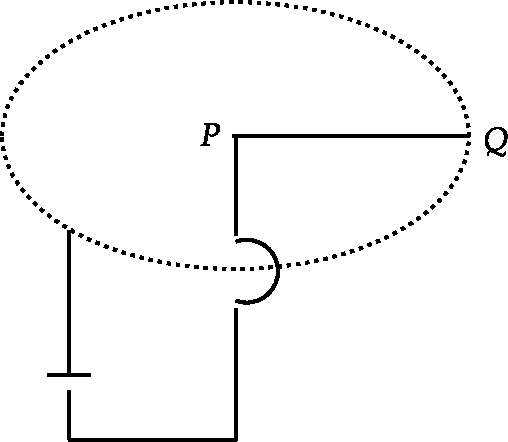
\includegraphics[width=3cm,height=3cm]{EM-18-crop}
		\end{center}
	\end{figure}
	\begin{tasks}(4)
		\task[\textbf{a.}]0
		\task[\textbf{b.}]$\frac{2 B I}{3 M}$
		\task[\textbf{c.}] $\frac{3 B I}{2 M}$
		\task[\textbf{d.}] $\frac{B I}{M}$
	\end{tasks}
	\item A particle of mass $m$ carrying charge $q$ is moving in a circle in a magnetic field $B$. According to Bohr's model, the energy of the particle in the $n^{\text {th }}$ level is{\exyear{IIT JAM 2014}}
	\begin{tasks}(4)
		\task[\textbf{a.}]$\frac{1}{n^{2}}\left(\frac{h q B}{\pi m}\right)$
		\task[\textbf{b.}] $n\left(\frac{h q B}{\pi m}\right)$
		\task[\textbf{c.}]  $n\left(\frac{h q B}{2 \pi m}\right)$
		\task[\textbf{d.}]  $n\left(\frac{h q B}{4 \pi m}\right)$
	\end{tasks}
	\item A positively charged particle, with a charge $q,$ enters a region in which there is a uniform electric field $\vec{E}$ and a uniform magnetic field $\vec{B},$ both directed parallel to the positive $y$ -axis. At $t=0,$ the particle is at the origin and has a speed $v_{0}$ directed along the positive $x$ -axis. The orbit of the particle, projected on the $x-z$ plane, is a circle. Let $T$ be the time taken to complete one revolution of this circle. The $y$ -coordinate of the particle at $t=T$ is given by{\exyear{IIT JAM 2015}}
	\begin{tasks}(4)
		\task[\textbf{a.}]$\frac{\pi^{2} m E}{2 q B^{2}}$
		\task[\textbf{b.}]$\frac{2 \pi^{2} m E}{q B^{2}}$
		\task[\textbf{c.}] $\frac{\pi^{2} m E}{q B^{2}}+\frac{v_{0} \pi m}{q B}$
		\task[\textbf{d.}]   $\frac{2 \pi m v_{0}}{q B}$
	\end{tasks}
	
	\item A conducting wire is in the shape of a regular hexagon, which is inscribed inside an imaginary circle of radius $R,$ as shown. A current $I$ flows through the wire. The magnitude of the magnetic field at the center of the circle is {\exyear{IIT JAM 2015}}
	\begin{figure}[H]
		\begin{center}
			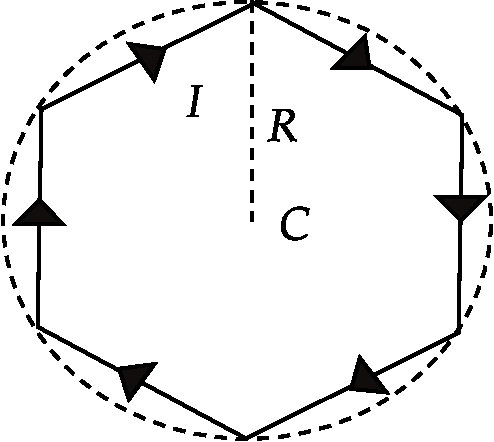
\includegraphics[width=2.5cm,height=2.5cm]{EM-26(q)-crop}
		\end{center}
	\end{figure}
	\begin{tasks}(4)
		\task[\textbf{a.}]$\frac{\sqrt{3} \mu_{0} I}{2 \pi R}$
		\task[\textbf{b.}]$\frac{\mu_{0} I}{2 \sqrt{3} \pi R}$
		\task[\textbf{c.}]$\frac{\sqrt{3} \mu_{0} I}{\pi R}$
		\task[\textbf{d.}] $\frac{3 \mu_{0} I}{2 \pi R}$
	\end{tasks}
	\item A charged particle in a uniform magnetic field $\vec{B}=B_{0} \hat{e}_{z}$ starts moving from the origin with velocity $\vec{v}=\left(3 \hat{e}_{x}+2 \hat{e}_{z}\right) m / s$. The trajectory of the particle and the time $t$ at which it reaches 2 meters above the $x y$-plane are ,$\left(\hat{e}_{x}, \hat{e}_{y}\right.$ and $\hat{e}_{z}$ are unit vectors in Cartesian-coordinate system){\exyear{IIT JAM 2016}}
	\begin{tasks}(2)
		\task[\textbf{a.}] Helical path; $t=1 s$
		\task[\textbf{b.}]Helical path; $t=2 / 3 s$
		\task[\textbf{c.}] Circular path; $t=1 s$
		\task[\textbf{d.}]  Circular path; $t=2 / 3 s$
	\end{tasks}
	\item Three infinitely-long conductors carrying currents $I_{1}, I_{2}$ and $I_{3}$ lie perpendicular to the plane of the paper as shown in the figure.If the value of the integral $\oint_{C} \vec{B} \cdot \overrightarrow{d l}$ for the loops $C_{1}, C_{2}$ and $C_{3}$ are $2 \mu_{0}, 4 \mu_{0}$ and $\mu_{0}$ in the units of $\frac{N}{A}$ respectively, then{\exyear{IIT JAM 2016}}
	\begin{figure}[H]
		\begin{center}
			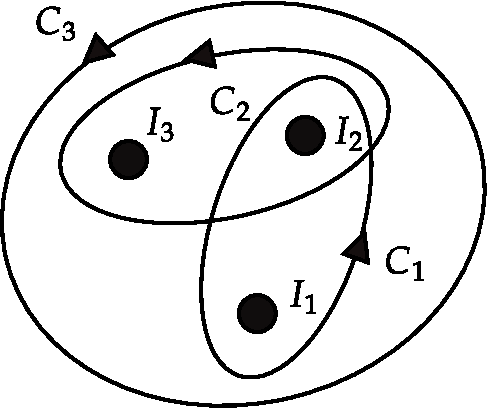
\includegraphics[width=3cm,height=2.5cm]{EM-44-crop}
		\end{center}
	\end{figure}
	\begin{tasks}(2)
		\task[\textbf{a.}]$I_{1}=3 A$ into the paper
		\task[\textbf{b.}] $I_{2}=5 A$ out of the paper
		\task[\textbf{c.}] $I_{3}=0$
		\task[\textbf{d.}] $I_{3}=1 A$ out of the paper
	\end{tasks}
	\item A current $I=10 A$ flows in an infinitely long wire along the axis of hemisphere (see figure). The value of $\int(\vec{\nabla} \times \vec{B}) \cdot \overrightarrow{d s}$ over the hemispherical surface as shown in the figure is:{\exyear{IIT JAM 2017}}
	\begin{figure}[H]
		\begin{center}
			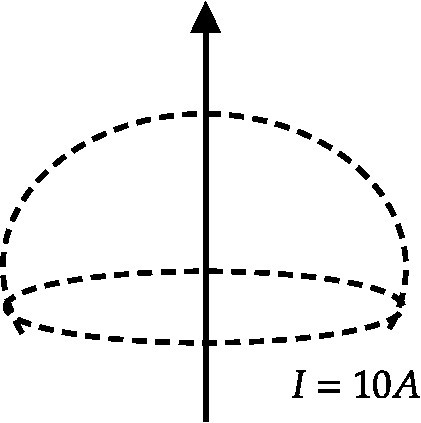
\includegraphics[width=3cm,height=3cm]{EM-46-crop}
		\end{center}
	\end{figure}
	\begin{tasks}(4)
		\task[\textbf{a.}]$10 \mu_{0}$
		\task[\textbf{b.}] $5 \mu_{0}$
		\task[\textbf{c.}]  0
		\task[\textbf{d.}] $7.5 \mu_{0}$
	\end{tasks}
	\item A current $I$ is flowing through the sides of an equilateral triangle of side $a$. The magnitude of the magnetic field at the centroid of the triangle is{\exyear{IIT JAM 2018}}
	\begin{figure}[H]
		\begin{center}
			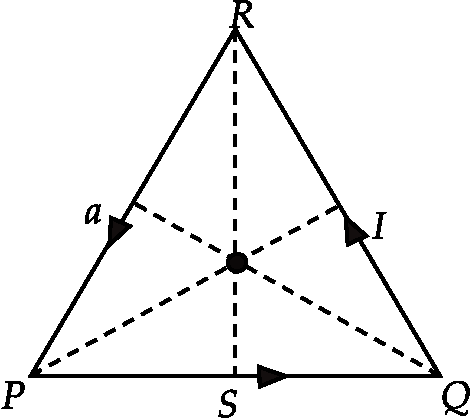
\includegraphics[width=3cm,height=2.5cm]{EM-57-crop}
		\end{center}
	\end{figure}
	\begin{tasks}(4)
		\task[\textbf{a.}]$\frac{9 \mu_{0} I}{2 \pi a}$
		\task[\textbf{b.}] $\frac{\mu_{0} I}{\pi a}$
		\task[\textbf{c.}]$\frac{3 \mu_{0} I}{2 \pi a}$
		\task[\textbf{d.}] $\frac{3 \mu_{0} I}{\pi a}$
	\end{tasks}
\end{enumerate}
\colorlet{ocre1}{ocre!70!}
\colorlet{ocrel}{ocre!30!}
\setlength\arrayrulewidth{1pt}
\begin{table}[H]
	\centering
	\arrayrulecolor{ocre}
	\begin{tabular}{|p{1.5cm}|p{1.5cm}||p{1.5cm}|p{1.5cm}|}
		\hline
		\multicolumn{4}{|c|}{\textbf{Answer key}}\\\hline\hline
		\rowcolor{ocrel}Q.No.&Answer&Q.No.&Answer\\\hline
		1&\textbf{b} &2&\textbf{c}\\\hline 
		3&\textbf{d} &4&\textbf{b}  \\\hline
		5&\textbf{c} &6&\textbf{a} \\\hline
		7&\textbf{a} and \textbf{b}&8&\textbf{a}\\\hline
		9&\textbf{a}& & \\\hline
		
	\end{tabular}
\end{table}
\begin{abox}
	Practise Set-2
\end{abox}
\begin{enumerate}[ label=\color{ocre}\textbf{\arabic*.}]
	\item The wire loop $P Q R S P$ formed by joining two semicircular wires of radii $R_{1}$ and $R_{2}$ carries a current $I$ as shown in the figure. Then the magnetic field $B$ at the centre is 
	\begin{figure}[H]
		\begin{center}
			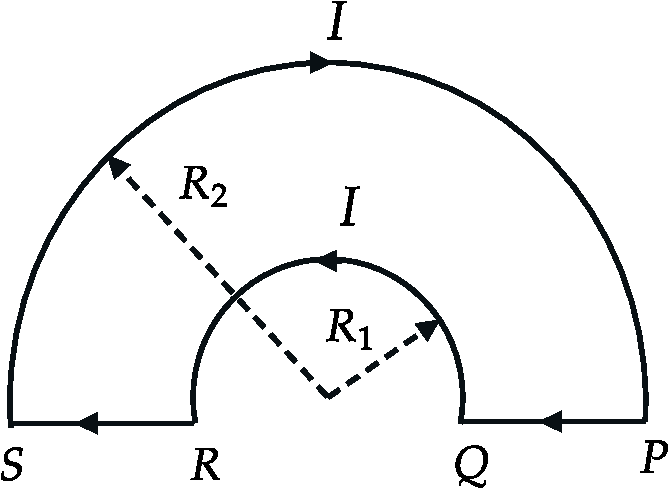
\includegraphics[width=3.5cm,height=2.5cm]{diagram-20210428(1)-crop}
		\end{center}
	\end{figure}
	\begin{tasks}(2)
		\task[\textbf{a.}] $\frac{\mu_{0} I}{2}\left(\frac{1}{R_{1}}-\frac{1}{R_{2}}\right)$, outward
		\task[\textbf{b.}]$\frac{\mu_{0} I}{2}\left(\frac{1}{R_{1}}-\frac{1}{R_{2}}\right)$, inward
		\task[\textbf{c.}] $\frac{\mu_{0} I}{4}\left(\frac{1}{R_{1}}-\frac{1}{R_{2}}\right)$, outward
		\task[\textbf{d.}]  $\frac{\mu_{0} I}{4}\left(\frac{1}{R_{1}}-\frac{1}{R_{2}}\right)$, inward.
	\end{tasks}
	\item A wire of circular cross section of radius $\mathrm{R}$ carries a volume current density $\mathrm{J}=\mathrm{kr}^{2} \hat{\mathrm{Z}}$ along the length of the wire. The magnetic field at a position $r<R$ is:
	\begin{tasks}(4)
		\task[\textbf{a.}] $\frac{\mu_{0}}{2} \mathrm{kr}^{3} \hat{\mathrm{z}}$
		\task[\textbf{b.}]$\frac{\mu_{0}}{4} \mathrm{k} \mathrm{r}^{3} \hat{\phi}$
		\task[\textbf{c.}] $\frac{\mu_{0}}{4 \pi} \mathrm{kr}^{3} \hat{\mathrm{r}}$ 
		\task[\textbf{d.}]  $\frac{\mu_{0}}{4 \pi} \mathrm{kr}^{2} \hat{\phi}$
	\end{tasks}
	\item A uniform surface current is flowing in the positive $y$ -direction over an infinite sheet lying in the $x-y$ plane. The direction of the magnetic field is:
	\begin{tasks}(1)
		\task[\textbf{a.}] Along $-\hat{z}$ for $z>0$ and along $\hat{z}$ for $z<0$
		\task[\textbf{b.}]Along $-\hat{x}$ for $z>0$ and along $\hat{x}$ for $z<0$
		\task[\textbf{c.}] Along $\hat{z}$ for $z>0$ and along $\hat{x}$ for $z<0$
		\task[\textbf{d.}] Along $\hat{x}$ for $z>0$ and along $-\hat{x}$ for $z<0$
	\end{tasks}
	\item In a conduction wire of radius $a$ carrying a volume current varies with the radial distance as $J=(\frac{r}{a})J_0$ is parallel to the axis. Calculate the total current through the wire 
	\begin{tasks}(4)
		\task[\textbf{a.}] $\frac{\pi}{3}a^3 J_0$
		\task[\textbf{b.}]$\frac{2\pi}{3}a^2 J_0$
		\task[\textbf{c.}] $\frac{2 \sqrt{2}\pi}{3}a^3 J_0$
		\task[\textbf{d.}]  $\frac{3 \sqrt{2}\pi a^2 J_0}{2}$
	\end{tasks}
	\item Find the magnetic field at $0$ for the following figures.
	\begin{tasks}(2)
		\task[\textbf{(a)}]	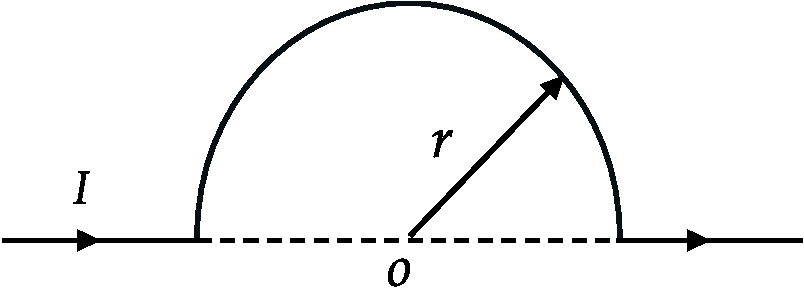
\includegraphics[width=4.5cm,height=2cm]{diagram-20210428(2)-crop} 
		\task[\textbf{(b)}] 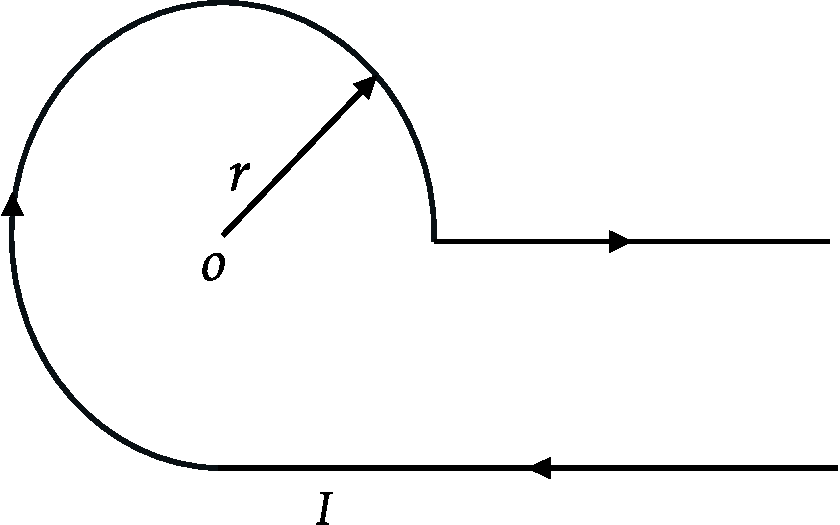
\includegraphics[width=4cm,height=2.5cm]{diagram-20210428(3)-crop} 
	\end{tasks}
	\begin{tasks}(2)
		\task[\textbf{a.}] $\frac{\mu_{0} I}{4r}$\ and\ $\frac{\mu_{0} I}{4\pi r}[1+\frac{3\pi}{2}]$
		\task[\textbf{b.}] $\frac{\mu_{0} I}{4r}$\ and\ $\frac{\mu_{0} I}{2\pi r}[1+\frac{3\pi}{4}]$
		\task[\textbf{c.}] $\frac{\mu_{0} I}{4r}$\ and\ $\frac{\mu_{0} I}{2\pi r}[1+\frac{\pi}{2}]$
		\task[\textbf{d.}] $\frac{\mu_{0} I}{4r}$\ and\ $\frac{\mu_{0} I}{\pi r}[2+\frac{3\pi}{4}]$
	\end{tasks}
	\item The wire is given a shape ABCD as shown in figure given below through which a steady current $I$ flows. The magnetic field at the centre $p$ is $\frac{\alpha\mu_{0} I}{r}$.Then the value of $\alpha$ is
	\begin{figure}[H]
		\begin{center}
			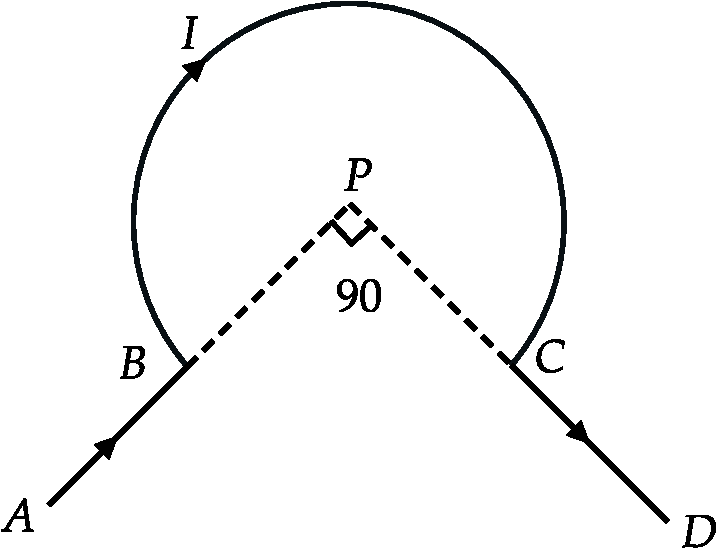
\includegraphics[width=4cm,height=3cm]{diagram-20210429(3)-crop}
		\end{center}
	\end{figure}
	\begin{tasks}(4)
		\task[\textbf{a.}]$\frac{1}{8}$
		\task[\textbf{b.}]$\frac{2}{8}$
		\task[\textbf{c.}]$\frac{3}{8}$
		\task[\textbf{d.}]  $\frac{5}{8}$
	\end{tasks}
	\item In a solenoid the magnetic field is maximum at 
	\begin{tasks}(4)
		\task[\textbf{a.}]  It's centre .
		\task[\textbf{b.}]  It's ends.
		\task[\textbf{c.}]Away from it. 
		\task[\textbf{d.}] None of these.
	\end{tasks}
	\item A large parallel plate capacitor with uniform surface charge $\sigma$ on the upper plate and $-\sigma$on the lower plate is moving with a constant speed $V$. Find the magnetic field between them.
	\begin{figure}[H]
		\begin{center}
			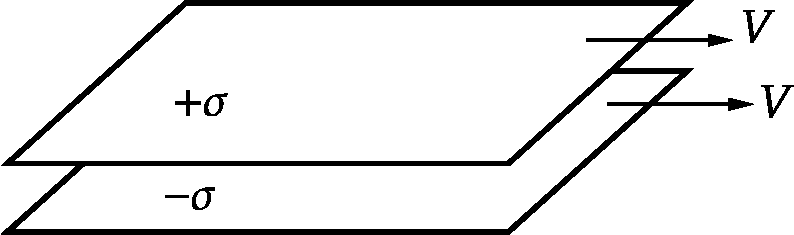
\includegraphics[width=4cm,height=2cm]{diagram-20210428(5)-crop}
		\end{center}
	\end{figure}
	\begin{tasks}(4)
		\task[\textbf{a.}]zero
		\task[\textbf{b.}]$\frac{\mu_{0}\sigma V}{2}$
		\task[\textbf{c.}]$\mu_{0} \sigma V$
		\task[\textbf{d.}] 2$\mu_{0}\sigma V$
	\end{tasks}
	\item Two long coaxial solenoids carry current $I$ but in opposite direction. The inner solenoid cradius $a$ has $n_1$ turns per unit length, and the outer one cradius $b$has $n_2$.Find $B$ inside the inner solenoid.
	\begin{figure}[H]
		\begin{center}
			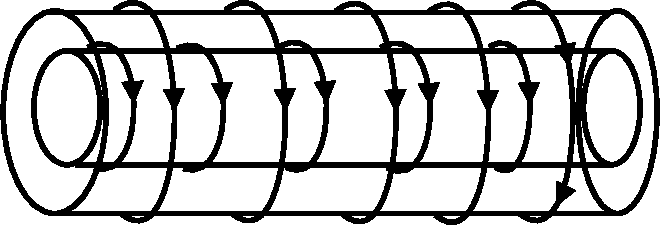
\includegraphics[width=5cm,height=2cm]{diagram-20210428(6)-crop}
		\end{center}
	\end{figure}
	\begin{tasks}(4)
		\task[\textbf{a.}]$\mu_{0}I(n_1-n_2)\hat{z}$
		\task[\textbf{b.}]$\mu_{0}I(n_2-n_1)\hat{z}$
		\task[\textbf{c.}]$\mu_{0}In_1\hat{z}$
		\task[\textbf{d.}] zero
	\end{tasks}
	\item In a cyclotron, $\alpha$particle are accelarated using $FF$sourcr of frequency $I5MH_Z$.
	What would be the frequency RF source if $\alpha$particles are replaced by $He^3$ particle.
	\begin{tasks}(4)
		\task[\textbf{a.}]$9 \ MHz$
		\task[\textbf{b.}]$12 \ MHz$
		\task[\textbf{c.}]$16\ MHz$
		\task[\textbf{d.}]$20\ MHz$
	\end{tasks}
	\item Two particle $X$ and $Y$ having equal charges. After being accelerated through the same potential difference enter a region of unifoem magnetic field and describe ancular path of radius $R_1$ and $R_2$ respectively. The ration of the man of $X$to that $Y$ is
	\begin{tasks}(4)
		\task[\textbf{a.}]$\sqrt{\frac{R_1}{R_2}}$
		\task[\textbf{b.}]$\sqrt{\frac{R_2}{R_1}}$
		\task[\textbf{c.}]$\sqrt{\frac{R_1}{R_2}}^2$
		\task[\textbf{d.}]${\frac{R_1}{R_2}}$
	\end{tasks}
	\item Astream of electrons enters, from left to right a uniform magnetic field $B$ which is pointing  a upward as shown in figure. The field deflect the stream of electrons.
	\begin{figure}[H]
		\begin{center}
			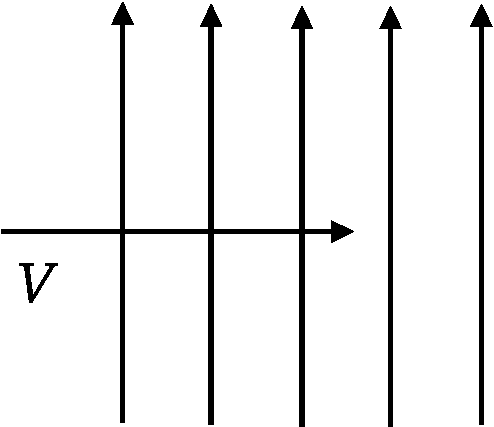
\includegraphics[width=3.5cm,height=2.5cm]{diagram-20210428(4)-crop}
		\end{center}
	\end{figure}
	\begin{tasks}(2)
		\task[\textbf{a.}]Downward(in the plane of the paper).
		\task[\textbf{b.}]Upward (in the plane of the paper).
		\task[\textbf{c.}]In to the paper.
		\task[\textbf{d.}]Out of the paper.
	\end{tasks}
	\item The electron move $s$ with velocity $\hat{V}=V_0 \hat{j}$ \ under the combined influence of $\vec{E}=E_0 \hat{i}$and $\vec{B}=-B_0 \hat{k}$ fields.The force on the electron is in the 
	\begin{tasks}(4)
		\task[\textbf{a.}]$Y$ \ direction
		\task[\textbf{b.}]$Z$ \ direction
		\task[\textbf{c.}]$YZ$ \ plane 
		\task[\textbf{d.}]$X$ \ direction
	\end{tasks}
	\item The chaged particle moves in a helical path under the influence of a constant magnetic field. The initial velocity is such that the component along the magnetic field is twice the component in the plane normal to the magnetic field. The ratio of pitch to the radius \ $R$ of the helical path is,
	\begin{tasks}(4)
		\task[\textbf{a.}]$\frac{\pi}{2}$
		\task[\textbf{b.}]$4\pi$
		\task[\textbf{c.}] $2\pi$
		\task[\textbf{d.}]$\pi$
	\end{tasks}
	\item A proton, dueteron and an $\alpha$ particle having the same $KE$ are moving in circular tajectories in a constant magnetic field. If $R_p,R_d,R_\alpha $ denote the radius respectively then
	\begin{tasks}(4)
		\task[\textbf{a.}]$R_p<R_d=R_\alpha$
		\task[\textbf{b.}]$R_\alpha=R_p>R_d$
		\task[\textbf{c.}]$R_\alpha>R_p<R_d$
		\task[\textbf{d.}]$R_\alpha=R_p=R_d$
	\end{tasks}
\end{enumerate}
\colorlet{ocre1}{ocre!70!}
\colorlet{ocrel}{ocre!30!}
\setlength\arrayrulewidth{1pt}
\begin{table}[H]
	\centering
	\arrayrulecolor{ocre}
	
	\begin{tabular}{|p{1.5cm}|p{1.5cm}||p{1.5cm}|p{1.5cm}|}
		\hline
		\multicolumn{4}{|c|}{\textbf{Answer key}}\\\hline\hline
		\rowcolor{ocrel}Q.No.&Answer&Q.No.&Answer\\\hline
		1&\textbf{c}&2&\textbf{b}\\\hline 
		3&\textbf{d}&4&\textbf{b}\\\hline
		5&\textbf{a}&6&\textbf{c}\\\hline
		7&\textbf{a}&8&\textbf{c}\\\hline
		9&\textbf{a}&10&\textbf{d}\\\hline
		11&\textbf{d}&12&\textbf{c}\\\hline
		13&\textbf{d}&14&\textbf{b}\\\hline
		15&\textbf{a}&&\\\hline
	\end{tabular}
\end{table}

\newpage
\begin{abox}
	Practise Set-3
\end{abox}
\begin{enumerate}[ label=\color{ocre}\textbf{\arabic*.}]
	\item Consider a coil of radius $R$ is placed in $XY$ plane having current $I$ passing through it. Auppose another coil having the same radius $R$ is placed at a distance $2R$ from the first. Find the magnetic field at the mid point between them?
	\begin{figure}[H]
		\begin{center}
			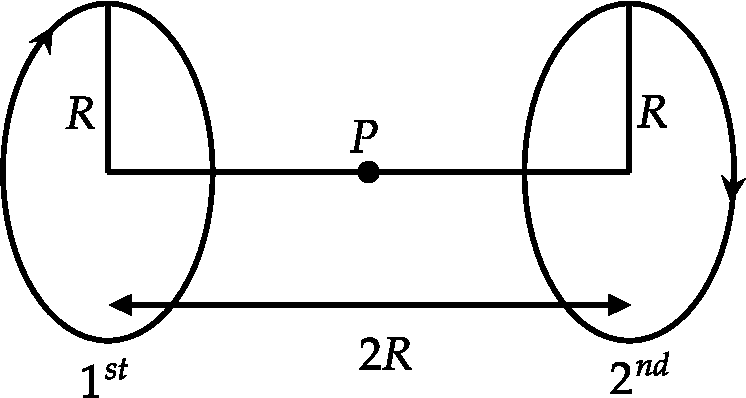
\includegraphics[width=4cm,height=2cm]{diagram-20210430-crop}
		\end{center}
	\end{figure}
	\begin{answer}
		\begin{align*}
		&B \text{at}\quad\text{is}=B_1+B_2\\
		B_1&=\frac{\mu_{0} I}{2}\times\frac{R^2}{(R^2+R^2)^\frac{3}{2}}\qquad \text{here,}\ z=R\\
		&=\frac{\mu_0 I}{2}\frac{R^2}{2^\frac{3}{2}\times R^3}=\frac{\mu_0 I}{2\times2^\frac{3}{2}\times R}\\
		B_2 \text{is also same}\\
		\therefore B&=2\times\frac{\mu_0 I}{2\times2^\frac{2}{3}R}=\frac{\mu_0I}{2\sqrt{2}R}
		\end{align*}
	\end{answer}
	\item  A very long solenoid with $n$ turns per unit length carries a current $I$. The magnetic field at a point which is on its axis and its end face?
	\begin{figure}[H]
		\begin{center}
			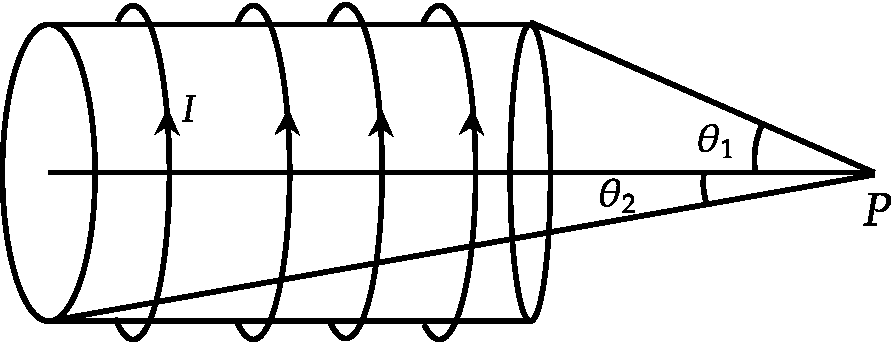
\includegraphics[width=6cm,height=2cm]{diagram-20210430(2)-crop}
		\end{center}
	\end{figure}
	\begin{answer}
		For a solenoid magnetic field at any point $P$ on its axis is given by
		$$B=\frac{\mu_0 nI}{2}(\cos\theta_2-\cos\theta_1)$$
		$\theta_1$ and $\theta_2$ are the angle made by the end points of the solenoid to $P$.\\
		\begin{align*}
		\therefore\text{In the case of infinite solenoid,at center}\\
		\theta_1&=\pi,\theta_2=0\\
		\therefore B&=\frac{\mu_0 nI}{2}\times2=\mu_0 nI \quad\text{at center}\\
		\text{Here in this question,at one end},\\
		\theta_1&=\frac{\pi}{2},\quad\theta_2=0 \text{(for long solenoid)}\\
		B&=\frac{\mu_0 n I}{2}\times1=\frac{\mu_0 n I}{2}
		\end{align*}
	\end{answer}
	\item A steady current $I$ flows down a long cylindrical wire of radius $a$ Find the magnetic field, both inside and outside the wire, if\\
	\textbf{(a)} The current is uniformly distributed over the outside surface of the wire.\\
	\textbf{(b)} The current is distributed in such a way that $J$ is proportional to $s$, the distance from the axis.
	\begin{figure}[H]
		\begin{center}
			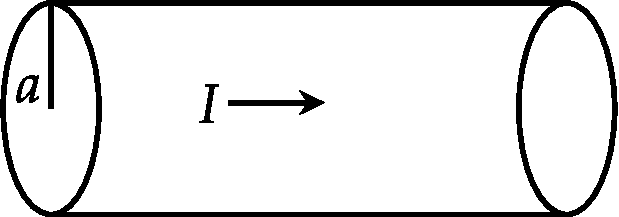
\includegraphics[width=3.5cm,height=1.5cm]{diagram-20210430(8)-crop}
		\end{center}
	\end{figure}
	\begin{answer}
		\textbf{(a)} Here current is uniform\\
		Inside the wire \quad $B=0$\quad $s<a$, no current enclosed \\
		outside the wire\quad $\oint B\cdot dl=\mu_0I$\\
		\begin{align*}
		dl&=2\pi s\\
		\text{s is the radius of }&\text{Amperial loop $dl$ around the wire}\\
		\therefore B\times2\pi s&=\mu_0I\\
		B&=\frac{\mu_0I}{2\pi s}s>a\\
		\end{align*}
		\textbf{(b)}
		\begin{align*}
		\text{inside the wire}
		J&=ks\\
		\text{First  we have to find }&\text{  $k$,so}\hspace{3cm}I=\text{total current}\\
		\text{We know}I&=\int_{0}^{a}J\cdot da \hspace{2cm}J=ks \quad da=2\pi s ds\\
		\therefore I&=k2\pi\int_{0}^{a}s^2ds\\
		I&=k2\pi s\frac{s^3}{3}\quad\text{so}\quad k=\frac{3I}{2\pi a^3}
		\intertext{Now inside the wire Consider an Amperial loop of radius \ $s$\ inside the wire}
		\text{So}\oint B\cdot dl&=\mu_0I \hspace{3cm}J=ks\\
		B\times2\pi s&=\mu_0I\hspace{3cm}ds=2\pi sds\\
		I=\int_{0}^{s}J.ds&=\int_{0}^{s}ks\times2\pi sds\\
		&=k\int_{0}^{s}s^2 ds\times2\pi\\
		&=\frac{ks^3}{3}\times2\pi\\
		\text{Substituting  value of }k\\
		I&=\frac{3 I}{2\pi a^3}\times\frac{s^3}{3}\times2\pi\\
		&=\frac{Is^3}{a^3}\\
		\therefore B\times2\pi s&=\frac{\mu_0Is^3}{a^3}\\
		B&=\frac{\mu_0Is^2}{2\pi a^3}\hat{\phi} \quad \text{inside}\\
		\text{Out side the wire}\\
		\oint B\cdot dl&=\mu_0I\\
		B\times2\pi s&=\mu_0I\\
		B&=\frac{\mu_0I}{2\pi s}\hat{\phi}
		\end{align*}
	\end{answer}
	\item Find the magnetic field at the center $O$ for the following figures.\\
	\begin{minipage}{0.45\textwidth}
		\begin{figure}[H]
			\begin{center}
				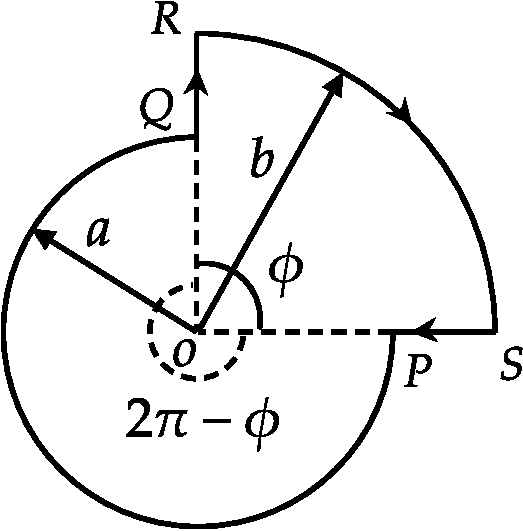
\includegraphics[width=3.5cm,height=3.5cm]{diagram-20210430(1)-crop}
			\end{center}
			\caption{(a)}
		\end{figure}
	\end{minipage}
	\begin{minipage}{0.45\textwidth}
		\begin{figure}[H]
			\begin{center}
				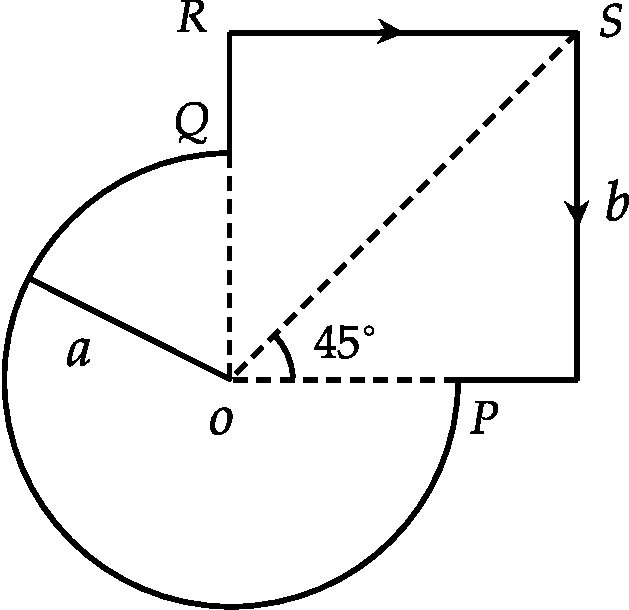
\includegraphics[width=3.5cm,height=3.5cm]{diagram-20210430(4)-crop}
			\end{center}
			\caption{(b)}
		\end{figure}
	\end{minipage}
	\begin{answer}
		\textbf{(a)}
		\begin{align*}
		\intertext{Field at $O$ due to $PS$ and $QR$ is zero. Because the point $O$ lies along the axis of the segment.}
		\text{Field at $O$ due to $RS$,}\\
		B_1&=\frac{\mu_0I}{2b}\times\frac{\phi}{2\pi}\\
		\text{Field at $O$ due to $PQ$}\\
		B_2&=\frac{\mu_0I}{2a}\times\frac{2\pi-\phi}{2\pi}\\
		\text{So total field at B}\\
		B&=B_1+B_2\\
		&=\frac{\mu_0I}{4\pi}\left( \frac{\phi}{b}+\frac{2\pi-\phi}{a}\right) \\
		\end{align*}
		\textbf{(b)}
		\begin{align*}
		\text{Field at $O$ due to arc $pQ$}\\
		B_1&=\frac{\mu_0I}{2a}\times\frac{3\frac{\pi}{2}}{2\pi}\\
		=&\frac{\mu_0I}{2a}\times\frac{3}{4}
		\intertext{Field at $O$ due to $PT$ \ and\ $QR$\ are zero. Field at $O$ due to $ST$ and $RS$.}
		B_2=\ B_3&=\frac{\mu_0I}{4\pi b}(\sin\theta_2-\sin\theta_1)\\
		&=\frac{\mu_0I}{4\pi b}\sin45\hspace{3cm}\theta_2=45,\quad \theta_{1}=0\\
		&=\frac{\mu_0I}{4\pi b}\times\frac{1}{\sqrt{2}}\\
		\intertext{Total field at \ $O$,}
		B&=B_1+B_2+B_3\\
		&=\frac{\mu_0I}{2a}\times\frac{3}{4}+2\times\frac{\mu_0}{4\pi b}\times\frac{1}{\sqrt{2}}\\
		&=\frac{\mu_0I}{4\pi}\left[\frac{3\pi}{2a}+\frac{\sqrt{2}}{b} \right] 
		\end{align*}
	\end{answer}
	\item Magnetic field at center $O$ due to a regular pentagon if $I$ current flowing through it and $R$ be the distance from each side to $O$.
	\begin{figure}[H]
		\begin{center}
			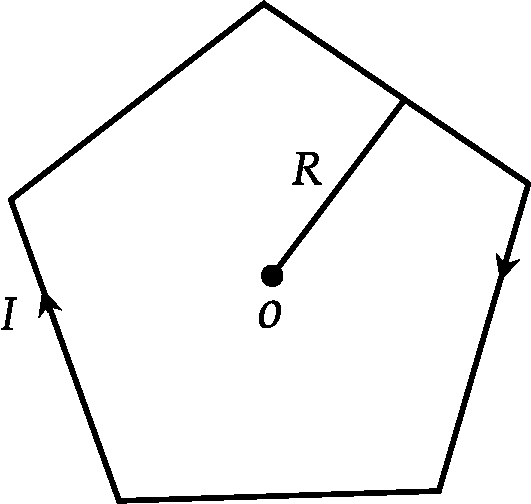
\includegraphics[width=2.5cm,height=2.5cm]{diagram-20210430(5)-crop}
		\end{center}
	\end{figure}
	\begin{answer}
		For an $n$ sided rectangular polygon field at center\\
		$B=\frac{n\mu_0I}{2\pi R}\tan\frac{\pi}{n}$ if $R$ become the distance from each vertex to center\\
		if $R$ is the distance from each side to center  
		\begin{align*}
		B&=\frac{n\mu_0I}{2\pi R}\sin\frac{\pi}{n}\\
		\text{Here,}\quad n&=5\quad \\
		\text{Then,} B&=\frac{\mu_0nI}{2\pi R}\sin\frac{\pi}{n}\\
		&=\frac{5\mu_0 I}{2\pi R}\sin\frac{\pi}{5}\\
		&=\frac{5\mu_0I}{2\pi R}\sin 36	
		\end{align*}
	\end{answer}
	\item Thick slab extending from $z=-a$ and $z=+a$ carries a uniform volume current $J=J(x) $.Find the magnetic field as a function of $Z$ both inside and outside the slab.
	\begin{figure}[H]
		\begin{center}
			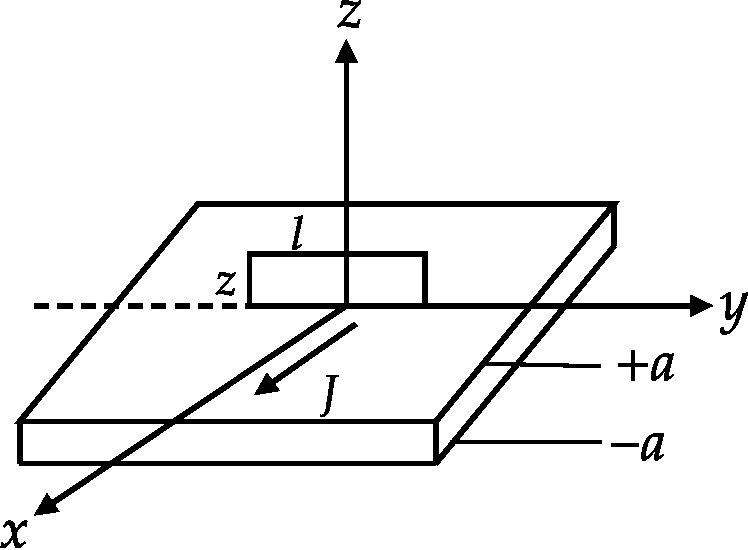
\includegraphics[width=5cm,height=3cm]{diagram-20210430(6)-crop}
		\end{center}
	\end{figure}
	\begin{answer}
		Consider an Amperian loop of length $l$ and height $z$, applying Ampere's law.\\
		\begin{align*}
		\oint B\cdot dl&=\mu_0I\\
		B\times l&=\mu_0\cdot lz\cdot J\hspace{3cm}I=lz\cdot \vec{J}\\
		\therefore B&=\mu_0Jz\hat{y}\hspace{3cm}(-a<z<a)\\
		\end{align*}
		By using right hand thumb rule we can say that for $z>0$ field is along $-y$ direction and for $z<0$ field is along $+y$ direction
		\begin{align*}
		\text{So}\quad B&=-\mu_0Ja\hat{y}\quad\text{for}\quad z>+a\\
		B&=+\mu_0Ja\hat{y}\quad\text{for}\quad z>-a
		\end{align*}
		By consideting an Amperian loop of length $l$ and height $a$.
	\end{answer}
	\item A beam of proton with velocity $4\times10^5 {m}/{Sec}$enters a uniform magnetic field of 0.3Tesla at an angle $60^\circ$to the magnetic field. Find the radius of the helical path taken by the proton beam. Also find the pitch of the helix.\\
	\begin{answer}
		\begin{align*}
		V&=4\times10^5 \frac{m}{Sec}\hspace{1cm}V_\perp=V\sin60\hspace{1cm}V_\parallel=V\cos60\\
		&\frac{mv_\perp^2}{R}=qv_\perp B\\
		R&=\frac{m v_\perp}{qB}\\
		&=0.012m \quad m_p=1.6\times 10^{-27}kg\\
		\text{Pitch of helix,}\\
		d&=V_\parallel T=V_\parallel\times\frac{2\pi m}{qB}=0.044m
		\end{align*}
	\end{answer}
	\item The maximum energy of deuteron coming out of a cyclotron accelerator is $20MeV$. The maximum energy of proton that can be obtained from the accelerator is?
	\begin{answer}
		\begin{align*}
		KE_{max}&=\frac{Q^2B^2R^2}{2m}\\
		KE_d&=20 MeV\\
		KE_P&=?\\
		20&=\frac{1\times B^2\times R^2}{2\times2}\\
		KE_P&=\frac{1\times B^2\times R^2}{2\times1}\\
		KE_P&=20MeV
		\end{align*}
	\end{answer}
	\item Ab $\alpha$ particle is accelerated by potencial difference of $10^4V$. Find the change in its direction of motion. If it enters normally in a region of thickness $0.1m$ having transverse magnetic induction of $0.1 $Tesla$(m=6.4\times10^-27kg)$
	\begin{figure}[H]
		\begin{center}
			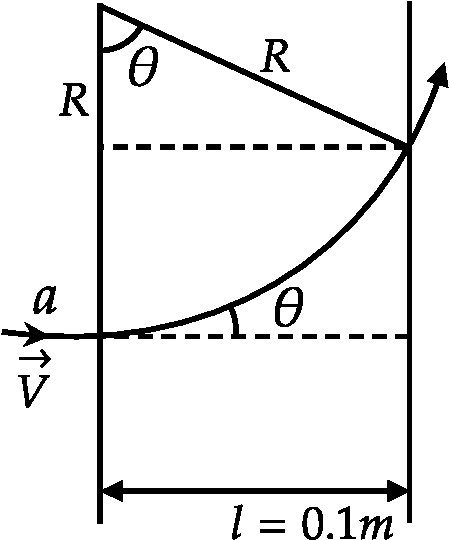
\includegraphics[width=3.5cm,height=2.5cm]{diagram-20210430(9)-crop}
		\end{center}
	\end{figure}
	\begin{answer}
		Before entering the field, $\alpha$ particle is accelerated by a potential difference of $10^4V$ then\begin{align*}
		\frac{1}{2}mu^2&=qV\\
		u&=\sqrt{\frac{2qV}{m}}\\
		R&=\frac{mu}{QB}=\frac{m}{QB}\sqrt{\frac{2qV}{m}}\quad V=pd\\
		&=\frac{1}{B}\sqrt{\frac{2mV}{q}}
		\intertext{$ \theta $ is the angle of deflection,}
		\therefore\sin\theta&=\frac{l}{R}\hspace{3cm}V=10^4\text{Volt}\\
		\sin\theta&=0.1\times B\times\sqrt{\frac{q}{2mV}}\\
		q&=2\times1.6\times10^{-16}=3.2\times10^{-16}c\\
		m=6.4\times10^{-27}kg\\
		\sin\theta&=0.1\times0.1\times\sqrt{\frac{3.2\times10^{-16}}{2\times6.4\times10^{-27}\times10^4}}\\
		&=\frac{1}{2}\\
		\therefore\theta&=30^\circ
		\end{align*}
	\end{answer}
	\item There are two similar coils at $P$ and $Q$ having same no of turns located at $(0,4,0)$ and$(0,0,3)$. Area of crone section are in the ratio $4:3$.A $16 A$ current flowing through coil $P$in clockwise direction and a $9\sqrt{3} A$ current in $Q$ in anticlockwise direction . What will the deflection of a compass needle placed at the origin. Assumes that earth field is negligible and radius of the coil are very small compared to their distance from the origin.
	\begin{figure}[H]
		\begin{center}
			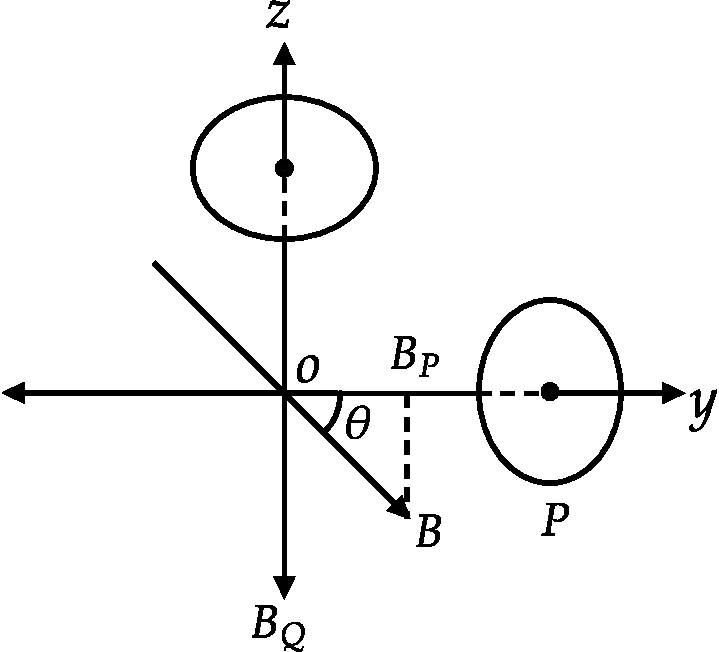
\includegraphics[width=5cm,height=4cm]{diagram-20210430(7)-crop}
		\end{center}
	\end{figure}
	\begin{answer}
		$B$ at a distance $x$ from a coil of radius $r$\\
		\begin{align*}
		B&=\frac{\mu_0I}{2}\frac{nr^2}{(r^2+x^2)^\frac{3}{2}}\\
		&=\frac{\mu_0 \ln \pi r^2}{2\times\pi \times(x^2)^\frac{3}{2}}\hspace{2cm}\quad \text{When}\ r<<<x\\
		&=\frac{\mu_0In\times A}{2\pi x^3}\\
		\text{Field at 'o' \ due to $P$},\\
		B_P&=\frac{\mu_0\times16\times A_P}{2\pi\times4^3}\\
		\text{Field at 'o' \ due to $Q$},\\
		B_Q&=\frac{\mu_0\times9\sqrt{3}\times A_Q}{2\pi\times3^3}\\
		\intertext{From figure resultant of \ $B_P$\ and \ $B_Q$,\ $B$ makes an angle With \ $B_Q$\ with \ $B_P$}\\
		\tan\theta&=\frac{B_Q}{B_P}
		=\frac{\mu_0\times9\sqrt{3} A_Q}{2\pi\times3^3}\times\frac{2\pi\times4^3}{\mu_0\times16\times A_P}\\
		\tan\theta&=\sqrt{3}\\
		\theta&=60^\circ
		\end{align*}
	\end{answer}
\end{enumerate}
\newpage
\begin{abox}
	Practise Set-1
\end{abox}
\begin{enumerate}[ label=\color{ocre}\textbf{\arabic*.}]
	\item A small loop of wire of area $A=0.01 \mathrm{~m}^{2}, N=40$ turns and resistance $R=20 \Omega$ is initially kept in a uniform magnetic field $B$ in such a way that the field is normal to the loop. When it is pulled out of the magnetic field, a total charge of $Q=2 \times 10^{-5} C$ flows through the coil. The magnitude of magnetic field $B$ is {\exyear{IIT JAM 2005}}
	\begin{tasks}(2)
		\task[\textbf{a.}]$1 \times 10^{-3} T$
		\task[\textbf{b.}]$4 \times 10^{-3} T$
		\task[\textbf{c.}]zero
		\task[\textbf{d.}] Unobtainable, as the data is insufficient
	\end{tasks}
	\item A uniform and constant magnetic field $B$ coming out of the plane of the paper exists in a rectangular region as shown in the figure. A conducting $\operatorname{rod} P Q$ is rotated about $O$ with a uniform angular speed $\omega$ in the plane of the paper. The emf $E_{P Q}$ induced between $P$ and $Q$ is best represented by the graph{\exyear{IIT JAM 2007}}
	\begin{figure}[H]
		\begin{center}
			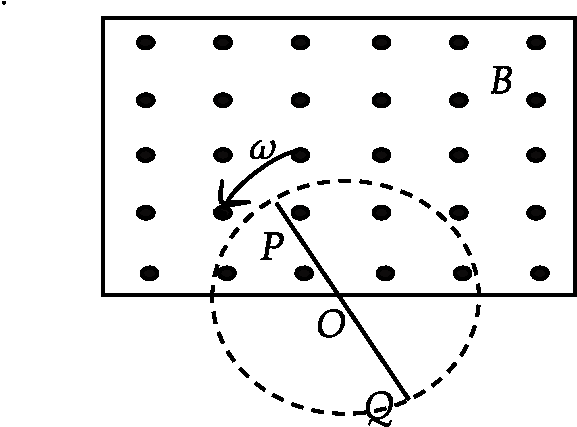
\includegraphics[width=3.5cm,height=3cm]{EM-05(q)-crop}
		\end{center}
	\end{figure}
	\begin{tasks}(2)
		\task[\textbf{a.}] 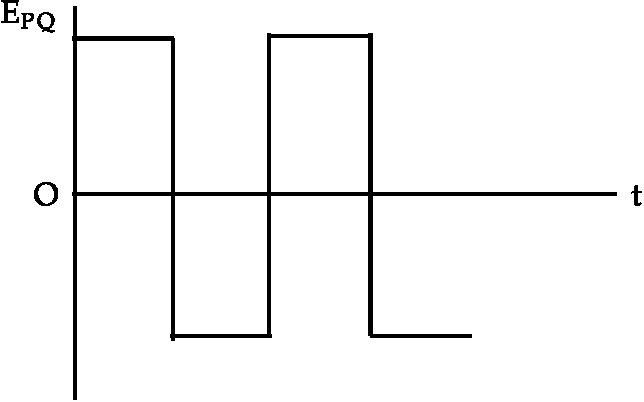
\includegraphics[width=3cm,height=2cm]{EM-05(a)-crop}
		\task[\textbf{b.}] 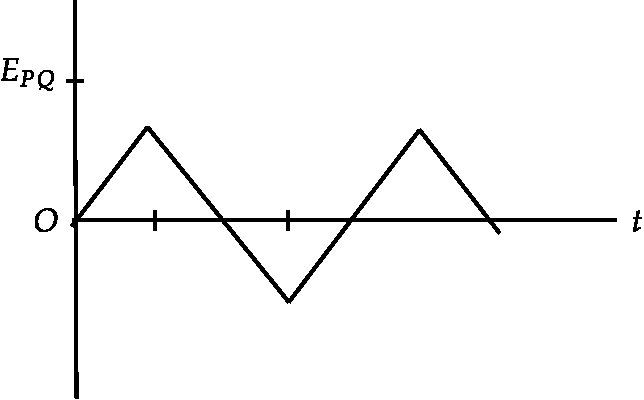
\includegraphics[width=3cm,height=2cm]{EM-05(b)-crop}
		\task[\textbf{c.}] 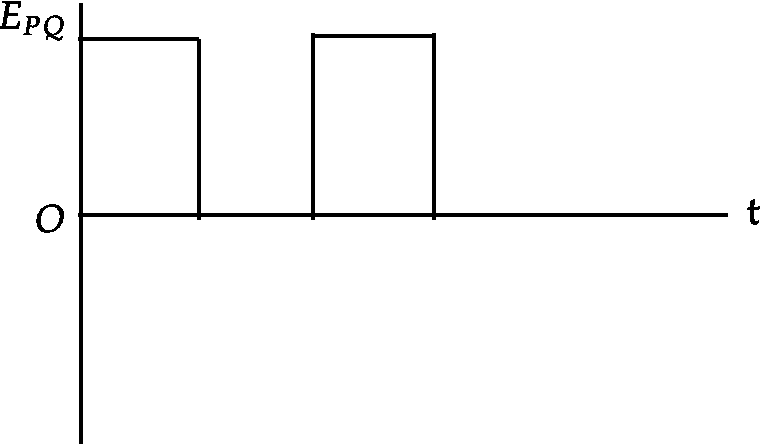
\includegraphics[width=3cm,height=2cm]{EM-05(c)-crop}
		\task[\textbf{d.}] 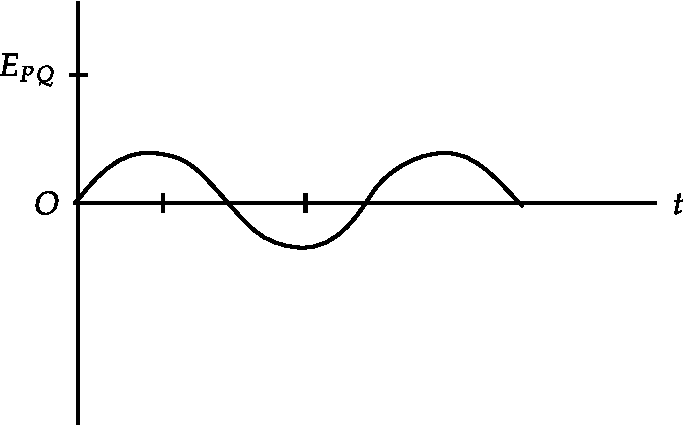
\includegraphics[width=3cm,height=2cm]{EM-05(d)-crop}
	\end{tasks}
	
	
	\item In a region of space, a time dependent magnetic field $B(t)=0.4 t$ tesla points vertically upwards. Consider a horizontal, circular loop of radius $2 \mathrm{~cm}$ in this region. The magnitude of the electric field $($ in $m V / m)$ induced in the loop is................{\exyear{IIT JAM 2015}}
	\item Consider a small bar magnet undergoing simple harmonic motion (SHM) along the $x$ - axis. A coil whose plane is perpendicular to the $x$ - axis is placed such that the magnet passes in and out of it during its motion. Which one of the following statements is correct? Neglect damping effects. {\exyear{IIT JAM 2016}}
	\begin{tasks}(1)
		\task[\textbf{a.}]Induced e.m.f. is minimum when the center of the bar magnet crosses the coil.
		\task[\textbf{b.}]The frequency of the induced current in the coil is half of the frequency of the SHM.
		\task[\textbf{c.}]Induced e.m.f. in the coil will not change with the velocity of the magnet.
		\task[\textbf{d.}] The sign of the e.m.f. depends on the pole $(N$ or $S$ ) face of the magnet which enters into the coil.
	\end{tasks}
	\item A rectangular loop of dimension $L$ and width $w$ moves with a constant velocity $v$ away from an infinitely long straight wire carrying a current $I$ in the plane of the loop as shown in the figure below. Let $R$ be the resistance of the loop. What is the current in the loop at the instant the near-side is at a distance $r$ from the wire?{\exyear{IIT JAM 2017}}
	\begin{figure}[H]
		\begin{center}
			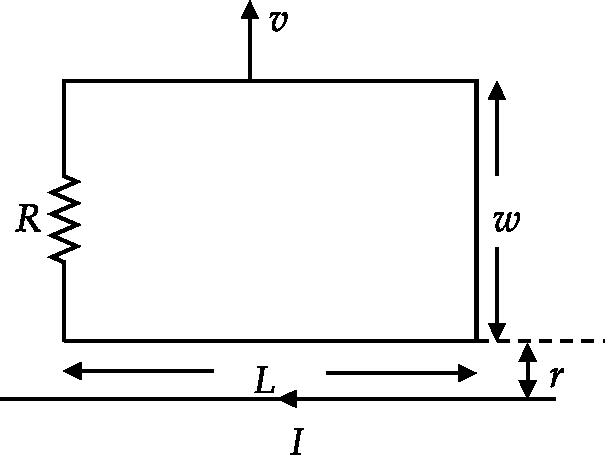
\includegraphics[width=3.5cm,height=3cm]{EM-50-crop}
		\end{center}
	\end{figure}
	\begin{tasks}(4)
		\task[\textbf{a.}] $\frac{\mu_{0} I L}{2 \pi R} \frac{w v}{r[r+2 w]}$
		\task[\textbf{b.}] $\frac{\mu_{0} I L}{2 \pi R} \frac{w v}{[2 r+w]}$
		\task[\textbf{c.}] $\frac{\mu_{0} I L}{2 \pi R} \frac{w v}{r[r+w]}$
		\task[\textbf{d.}]$\frac{\mu_{0} I L}{2 \pi R} \frac{w v}{2 r[r+w]}$
	\end{tasks}
	
	\item Consider two, single turn, co-planar, concentric coils of radius $R_{1}$ and $R_{2}$ with $R_{1} > R_{2}$. The mutual inductance between the two coils is proportional to{\exyear{IIT JAM 2017}}
	\begin{figure}[H]
		\begin{center}
			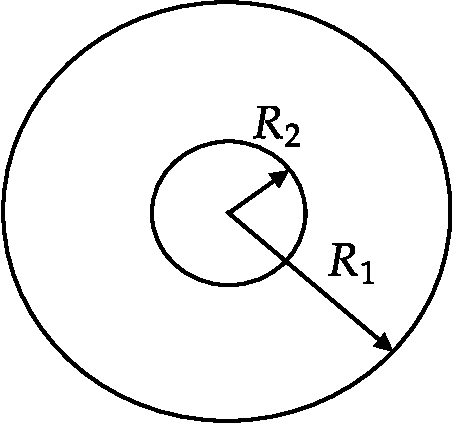
\includegraphics[width=3cm,height=3cm]{EM-47-crop}
		\end{center}
	\end{figure}
	\begin{tasks}(4)
		\task[\textbf{a.}]$\frac{R_{1}}{R_{2}}$
		\task[\textbf{b.}]$\frac{R_{2}}{R_{1}}$
		\task[\textbf{c.}]$\frac{R_{2}^{2}}{R_{1}}$
		\task[\textbf{d.}]$\frac{R_{1}^{2}}{R_{2}}$
	\end{tasks}
	\item A rectangular loop of dimensions $l$ and $w$ moves with a constant speed of $v$ through a region containing a uniform magnetic field $B$ directed into the paper and extending a distance of $4 w$. Which of the following figures correctly represents the variation of $\operatorname{emf}(\varepsilon)$ with the position $(x)$ of the front end of the loop?{\exyear{IIT JAM 2018}}
	\begin{figure}[H]
		\begin{center}
			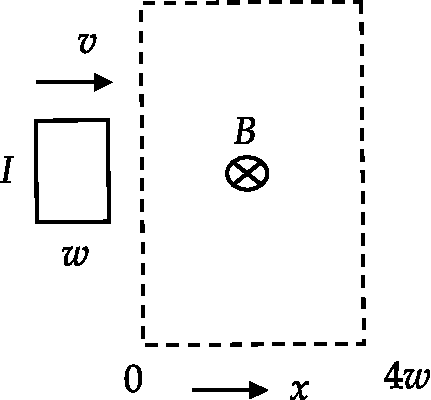
\includegraphics[width=3.5cm,height=3cm]{EM-59(q)-crop}
		\end{center}
	\end{figure}
	\begin{tasks}(2)
		\task[\textbf{a.}] 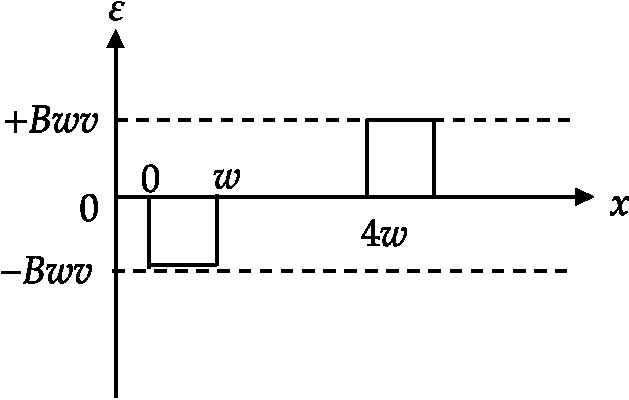
\includegraphics[width=3.5cm,height=2.5cm]{EM-59(a)-crop}
		\task[\textbf{b.}] 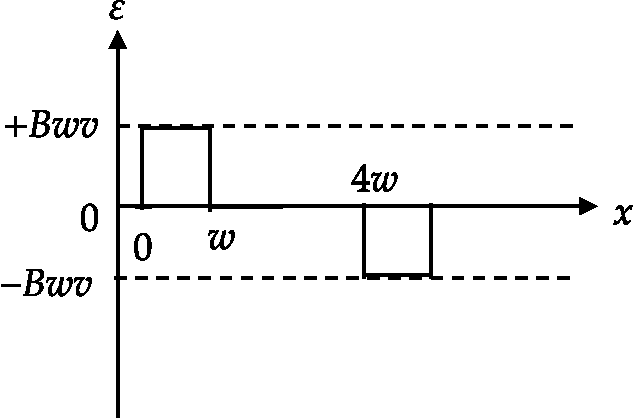
\includegraphics[width=3.5cm,height=2.5cm]{EM-59(b)-crop}
		\task[\textbf{c.}] 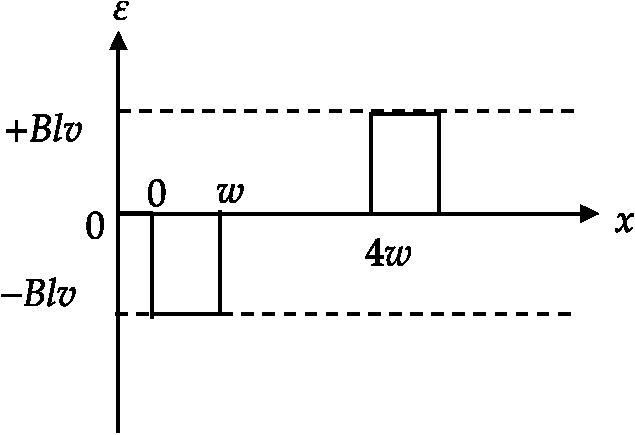
\includegraphics[width=3.5cm,height=2.5cm]{EM-59(c)-crop}
		\task[\textbf{d.}] 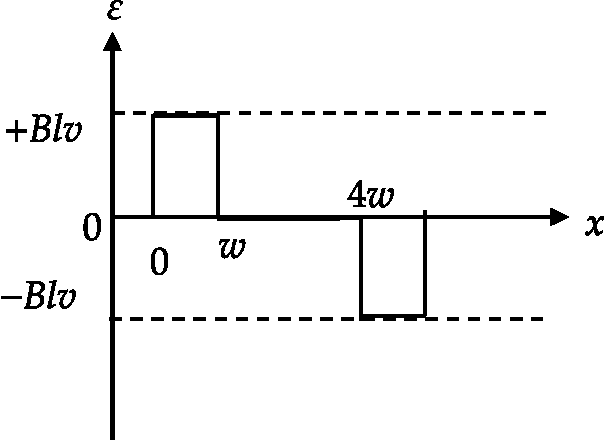
\includegraphics[width=3.5cm,height=2.5cm]{EM-59(d)-crop}
	\end{tasks}
\end{enumerate}
\colorlet{ocre1}{ocre!70!}
\colorlet{ocrel}{ocre!30!}
\setlength\arrayrulewidth{1pt}
\begin{table}[H]
	\centering
	\arrayrulecolor{ocre}
	\begin{tabular}{|p{1.5cm}|p{1.5cm}||p{1.5cm}|p{1.5cm}|}
		\hline
		\multicolumn{4}{|c|}{\textbf{Answer key}}\\\hline\hline
		\rowcolor{ocrel}Q.No.&Answer&Q.No.&Answer\\\hline
		1&\textbf{a} &2&\textbf{a}\\\hline 
		3&4 &4&\textbf{a} \\\hline
		5&\textbf{c} &6&\textbf{c} \\\hline
		7&\textbf{c}& &\\\hline
		
	\end{tabular}
\end{table}
\newpage
\begin{abox}
	Practise Set-2
\end{abox}
\begin{enumerate}[ label=\color{ocre}\textbf{\arabic*.}]
	\item A conducting rod of length $l$ rotates with a constant angular velocity as about its perpendicular bisector. An external uniform field $E$ is applied parallel to the axis of rotation. The potential difference  between the two ents of the rod is.
	\begin{tasks}(4)
		\task[\textbf{a.}]$\frac{1}{2}B\omega l^2$
		\task[\textbf{b.}]$\frac{1}{4}B\omega l^2$
		\task[\textbf{c.}]$B\omega l^2$
		\task[\textbf{d.}]$=zero$
	\end{tasks}
	\item A circular loop of radius $r$ is lying in the $xy$ plane with its center at the origin. If these exist a time varying magnetic field $B(t)=B_0^{-2t} \hat{z}(B_0<>0,2>0)$. Then the induced $emf$ in the loop.
	\begin{tasks}(4)
		\task[\textbf{a.}]-$\pi r^22B_0e^{-2t}$
		\task[\textbf{b.}]-$\pi r^2 B_0 e^{-2t}$
		\task[\textbf{c.}]$\pi r^2 B_0 e^{-2t}$
		\task[\textbf{d.}]$\pi r^22B_0e^{-2t}$
	\end{tasks}
	\item A large circular coil $N$ turns and radius $R$ carries a current $I=I_0\sin\omega t$. Another coil of small radius $r$ and $n$ turns is placed at the center of the large coil such that the coil are concentric and coplanar. The induced $emf$ in the coil?
	\begin{tasks}(1)
		\task[\textbf{a.}]Leads the current in the large coil by $\frac{\pi}{2}$
		\task[\textbf{b.}]Lags the current in large coil by $\pi$
		\task[\textbf{c.}]Is in phase with current in the large coil
		\task[\textbf{d.}]Lags the current in the large coil by $\frac{\pi}{2}$
	\end{tasks}
	\item Lenz's law is a concequence of the law of conservation of 
	\begin{tasks}(4)
		\task[\textbf{a.}]Charge 
		\task[\textbf{b.}]Energy 
		\task[\textbf{c.}]Momentum
		\task[\textbf{d.}]Mass
	\end{tasks}
	\item A long solenoid of radius $a$ carrying an alternating current $B(t)=B_0cos(\omega t)\hat{z}$. A circular loop of a wire of radius $\frac{a}{2}$and resistance $\hat{R}$ is placed inside the soleniod coaxial with it. Find the current induced in the loop?
	\begin{tasks}(4)
		\task[\textbf{a.}]$\frac{\pi a^2\omega B_0 \cos\omega t}{4R}$ 
		\task[\textbf{b.}]$\frac{\pi a^2\omega B_0 \sin\omega t}{4R}$ 
		\task[\textbf{c.}]$\frac{\pi a^2\omega B_0 \cos\omega t}{4R}$ 
		\task[\textbf{d.}]$\frac{\pi a^2\omega B_0 \sin\omega t}{2R}$ 
	\end{tasks}
	\item The current paning through a choke cod of $lH$ is decreasing at the rate $2A/sec$. Then $emf$ developed in the coil?
	\begin{tasks}(4)
		\task[\textbf{a.}]$2V$
		\task[\textbf{b.}]$0.5V $
		\task[\textbf{c.}]$-2V$
		\task[\textbf{d.}]$-0.5V$
	\end{tasks}
	\item Two inductors $L_1$and $L_2$are connected in series. The total inductance $L$\ will be
	\begin{tasks}(4)
		\task[\textbf{a.}]$L=L_1+L_2$
		\task[\textbf{b.}]$L=L_1+L_2+2m$
		\task[\textbf{c.}]$L=L_1+L_2+m$
		\task[\textbf{d.}]$L=L_1+L_2-m$
	\end{tasks}
	\item An infinitely long wire carrying a current $I(t)=I_0\cos\omega t$\ placed at a distance from a squar loop of side as shown in the figure. If the resistance of the loop is $R.$ Then the amplitude of the induced current in the loop?
	\begin{figure}[H]
		\begin{center}
			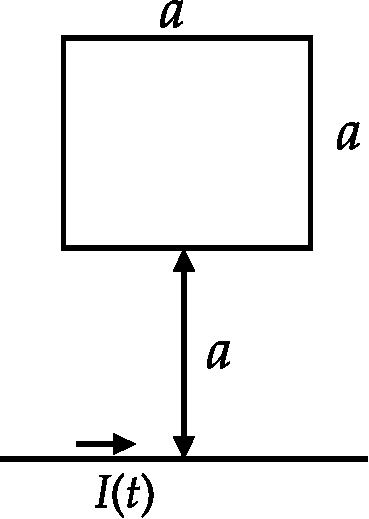
\includegraphics[width=3cm,height=3cm]{diagram-20210503-crop}
		\end{center}
	\end{figure}
	\begin{tasks}(4)
		\task[\textbf{a.}]$\frac{\mu_0}{2\pi}\frac{aI_0\omega}{R}\ln 2$
		\task[\textbf{b.}]$\frac{\mu_0}{\pi}\frac{aI_0\omega}{R}\ln 2$
		\task[\textbf{c.}]$\frac{\mu_0}{R}\frac{aI_0\omega}{R}\ln 2$
		\task[\textbf{d.}]$\frac{\mu_0}{2\pi}\frac{aI_0\omega}{R}$
	\end{tasks}
	\item A magnetic field $B$ is $B\hat{z}$\ direction $x>0$\ and zero elsewhere. A rectangular loop in the $xy$ \ plane of sides $l$\ (along$x$direction) is inserted in to the $x>0$\  region from the $x<0$\ region at a constant velocity $v=v\hat{x}$. Which of the following values of $l$\ and $h$\  will generate the largest EMF?
	\begin{tasks}(4)
		\task[\textbf{a.}]$l=8,h=3$
		\task[\textbf{b.}]$l=4,h=6$
		\task[\textbf{c.}]$l=6,h=4$
		\task[\textbf{d.}]$l=12,h=2$
	\end{tasks}
	\item The current in a $40mh$ inductor is given by $I=I_0 e^{-bt}$\ where $I_0=10A$\ and $b=20s^{-1}$. The magnitude of the inductor emf  at $t=25ms$\ is-------?
	\begin{tasks}(4)
		\task[\textbf{a.}]$3.7V$
		\task[\textbf{b.}]$4.8V$
		\task[\textbf{c.}]$5.5V$
		\task[\textbf{d.}]$1.6V$
	\end{tasks}
	\item Aconducting disc of radius is rotating about its own axis with a constant angular velocity $\omega$ in a uniform magnetic field acting perpendicular to the plane of the disc. Find the value of $emf$ induced between the rim and the center of the disc?
	\begin{tasks}(4)
		\task[\textbf{a.}]zero
		\task[\textbf{b.}]$\frac{1}{2}Ba^2\omega$
		\task[\textbf{c.}]$\frac{Ba^2\omega}{4}$
		\task[\textbf{d.}]$Ba^2\omega$
	\end{tasks}
	\item A conducting rod of length $l$ is rotated with uniform angular velocity $\omega$\ about one end in  a uniform magnetic field $B$. Electric field inside the rod at a distance $x$ from fixed end is?
	\begin{tasks}(4)
		\task[\textbf{a.}]$\omega Bx$
		\task[\textbf{b.}]$\frac{1}{2}\omega Bx$
		\task[\textbf{c.}]$\omega Bx^2$
		\task[\textbf{d.}]$\frac{1}{2}B\omega x^2$
	\end{tasks}
	\item A conducting wire of length $l$ is lying in $xy$ plane making $\theta$ angle with $x$ direction. It is translated with velocity $\vec{x}=\mu_0\hat{J}$. If there is a magnetic field $B=B_1 \hat{i}+B_2\hat{j}+B_3 \hat{k}$ in space. Motional $emf$ between the ends of rod is ?
	\begin{tasks}(2)
		\task[\textbf{a.}]Zero if $\theta$  \ is \ $90^\circ$
		\task[\textbf{b.}]Zero if $\theta=90^\circ$\ and\ $B_2=0$
		\task[\textbf{c.}]Zero if $\theta\neq90^\circ$\ and\ $B_3=0$
		\task[\textbf{d.}]Independent of \ $B$
	\end{tasks}
	\item A metallic ring of area $1cm^2$ and a resistance $10$ is placed in a $\perp^r$ time varying magnetic field which has the following form,
	$$B(t)=2e^{-0.5t}\cos(2\pi t)$$where $B$\ is in tesla and it is in seconds. The net charge that flows past any point in the ring form $t=0$ to $t=\alpha$ 
	\begin{tasks}(4)
		\task[\textbf{a.}]$1\mu c$
		\task[\textbf{b.}]$3\mu c$
		\task[\textbf{c.}]$5\mu c$
		\task[\textbf{d.}]$20\mu c$
	\end{tasks}
	\item The $SI$ unit of inductance, the henry can be written as.
	\begin{tasks}(4)
		\task[\textbf{a.}]$\frac{webber}{Ampere}$
		\task[\textbf{b.}]$\frac{volt \ second }{Ampere}$
		\task[\textbf{c.}]$\frac{Joule}{(Ampere)^2}$
		\task[\textbf{d.}]$\frac{ohm}{second}$
	\end{tasks}
\end{enumerate}
\colorlet{ocre1}{ocre!70!}
\colorlet{ocrel}{ocre!30!}
\setlength\arrayrulewidth{1pt}
\begin{table}[H]
	\centering
	\arrayrulecolor{ocre}
	\begin{tabular}{|p{1.5cm}|p{1.5cm}||p{1.5cm}|p{1.5cm}|}
		\hline
		\multicolumn{4}{|c|}{\textbf{Answer key}}\\\hline\hline
		\rowcolor{ocrel}Q.No.&Answer&Q.No.&Answer\\\hline
		1&\textbf{d} &2&\textbf{d}\\\hline 
		3&\textbf{a} &4&\textbf{b} \\\hline
		5&\textbf{b} &6&\textbf{a} \\\hline
		7&\textbf{b}&8&\textbf{a}\\\hline
		9&\textbf{b}&10&\textbf{b}\\\hline
		11&\textbf{b} &12&\textbf{a}\\\hline
		13&\textbf{a,c,d}&14&\textbf{d}\\\hline
		15&\textbf{a}& &\\\hline
		
	\end{tabular}
\end{table}	

\newpage
\begin{abox}
	Practise Set-3
\end{abox}
\begin{enumerate}[ label=\color{ocre}\textbf{\arabic*.}]
	\item A squar loop of sid $a$ is pulled out of a constant perpendicular magnetic field B with constant velocity $v$. If the direction of velocity is parallel to one of its side and resistance of the loop is $R$. Work done in the proces.\\
	\begin{answer}
		\begin{align*}
		\operatorname{emf}\  \varepsilon&= Blv\sin\theta \hspace{3cm} \theta=90\\
		\varepsilon&=B l v  \hspace{3.2cm} \text{Here, }\ l=a\\
		\therefore \varepsilon&=B a v\\
		I&=\frac{V}{R}\\
		I&=\frac{B a v}{R}\\
		\text{Work done during the proces is to }&\text{stored as energy.}\\
		w&=\frac{1}{2} L I^{2}\\
		\text{We know,}\\
		\phi&=L I\\
		\text{Here } \phi&=B \cdot A=B  a^{2}\\
		B a^{2}&=L I\\
		L&=\frac{B a^{2}}{I}=\frac{B a^{2} \times R}{B a v}=\frac{a R}{v}\\
		\text{Work} &=\frac{1}{2} L I^{2}\\
		&=\frac{1}{2} \frac{a R}{v} \times \frac{B^{2} a^{2} v^{2}}{R^{2}}\\
		&=\frac{B^{2} a^{3} v}{2 R}
		\end{align*}
	\end{answer}
	\item The magnetic flux density in a region is given by $B=(2\hat{i}+3 \hat{j} -4 \hat{k}) e^{-2 t} w b / m^{2}$. A squar loop of $2 m$ side is placed in the region with its center at the origin and its sider along the co-ordinate axis (x,y). The emf Induced in the loop at $t=1 \sec$ is\\
	\begin{answer}
		\begin{align*}
		\phi&=B \cdot A\\
		\varepsilon&=\frac{-d \phi}{d t}=\frac{d B}{d t} \cdot A\\
		B&=(2\hat{i}+3 \hat{j} -4 \hat{k})e^{-2 t}\\
		\text{Since loop lies in $x,y$  }&\text{ plane  consider only $z$ component}\\
		B(z)&=-4 e^{-2 t}\\
		\varepsilon&=-\frac{d} {dt}(-4 e^{-2 t}\cdot A) \hspace{3cm}A=a^{2}\\
		&=4 \times 2 \times e^{-2 t} \times 4\hspace{2.7cm}=2^{2}=4\\
		\varepsilon&=8 \times 4 \times e^{-2 t}\\
		&=32 e^{-2 t}\\
		\varepsilon \text{ at } t&=1 \mathrm{sec}\\
		\varepsilon&=3 \times e^{-2}=0.41v
		\end{align*}
	\end{answer}
	\item There are two conductors seperated by a distance $a$ carrying a current $I$ in opposite direction. Suppose current is increasing at a rate, $\frac{dI}{dt}$ in both. A square loop of side a placed at a distance a from $a$ from one of the wire. Find the induced $emf$ in the squar loop and what is the direction of current?
	\begin{figure}[H]
		\begin{center}
			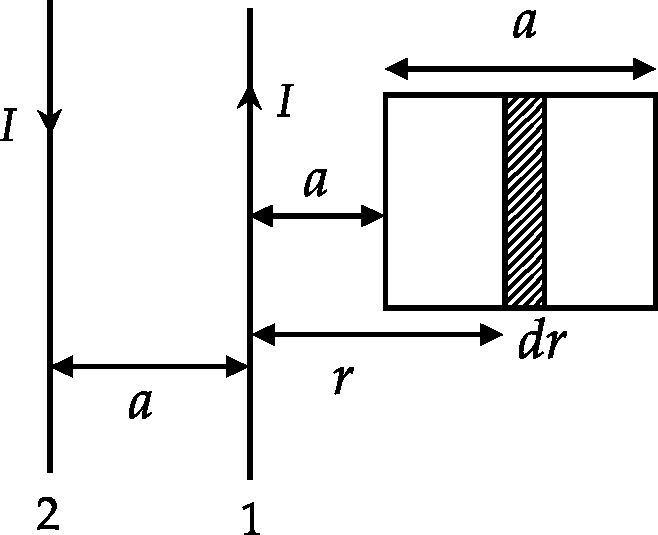
\includegraphics[width=4cm,height=3.5cm]{diagram-20210430(10)-crop}
		\end{center}
	\end{figure}
	\begin{answer}
		\begin{align*}
		\text{Field at a distance $r$ from the first wire}\\
		B_1&=\frac{\mu_0I}{2\pi r}\\
		\therefore \text{flux through $a\ dr$}\\
		d\phi_1&=B_1\cdot adr\\
		&=\frac{\mu_0Iadr}{2\pi r}\\
		\text{Total flux}\\
		d\phi&=\frac{\mu_0Ia}{2\pi}\int_{a}^{2a}\frac{1}{r}d
		r\\
		\phi_1&=\frac{\mu_0Ialn2}{2\pi}\\
		d\phi_2&=B_2\cdot adr\\	
		\phi_2&=\frac{\mu_0Ia}{2\pi}ln\frac{3}{2}\quad \text{Here } B_2=\frac{\mu_0I}{2\pi (r+a)}\\
		\therefore\text{Total flux}	 {\phi}&=\phi_1-\phi_2\\&=\frac{\mu_0Ia}{2\pi}ln\frac{4}{3}\\
		\text{Pointing into the page since $B_1$\ is higher.}\\
		\therefore\varepsilon&=\frac{-d\phi}{dt}=\frac{-\mu_0 a}{2\pi}ln\frac{4}{3}\frac{dI}{dt}
		\end{align*}
		According to Lenz's law the direction of induced current will be such that it opposes the change in flux .Therefore so current in the loop must flow in anticlockwise direction.
	\end{answer}
	\item A small loop of wire at area $A=0.01m^2,N=40$ turns and resintance $R=40$ is initially kept in a uniform magnetic field is such a way that the field is normal to the loop. When it is pulled out of the magnetic field a total charge of $Q=2\times10^{-5}C$ flows through the coil. The magnetic field\ $B=\cdots  \times10^{-3}$\ Tesla.\\
	\begin{answer}
		The induced emf , $\varepsilon$,\\
		\begin{minipage}{0.60\textwidth}
			\begin{align*}
			\varepsilon&=\frac{-d\phi}{dt}\\
			IR&=\frac{-d\phi}{dt}\\
			\frac{dQ}{dt}R&=\frac{dB}{dt}NA\\
			dQR&=BNA\\
			B&=\frac{dQ\times R}{A\times N}\\
			&=\frac{2\times10^{-5}\times40}{40\times0.01}\\
			&=2\times10^{-3}\ Tesla
			\end{align*}
		\end{minipage}
		\begin{minipage}{0.40\textwidth}
			\begin{align*}
			A&=0.01m^2\\
			N&=40\\
			R&=40\\
			Q&=2\times10^{-5}\\
			\varepsilon&=IR\\
			I&=\frac{dq}{dt}\\
			\phi&=BNA
			\end{align*}
		\end{minipage}
	\end{answer}
	\item A conducting circular loop is placed in a uniform magnetic field of $0.02$Tesla with its plane $\perp^r$\ to the field. If the radius of the loop starts shrinking at constant rate $1.0\ mm \ sec,$ \ Then the magnitude of $emf$ induced in the loop at the instant when the radius \ $4.0cm$\ will be -------$\mu_0$V\\
	\begin{answer}
		\begin{align*}
		\varepsilon&=\frac{-d\phi}{dt}\\
		\phi&=BNA\\
		\varepsilon&=\frac{-d\phi}{dt}=-BN\frac{dA}{dt}\\
		&=-BN\times2\pi r\times\frac{dr}{dt} \quad A=\pi r^2\\
		&=0.02\times2\times\frac{22}{7}\times4\times1\times10^{-3}\times10^{-2}\\
		&=5\times10^{-6}V\\&=5\mu V
		\end{align*}
	\end{answer}
	\item A metal bar of mass $m$ sides frictionlessly on two parallel conducting rails a distance $l$ a part. A resistor $R$ is connected across the rails and a uniform magnetic field $B$, pointing in to the page fills the entire region,  \\
	\begin{figure}[H]
		\begin{center}
			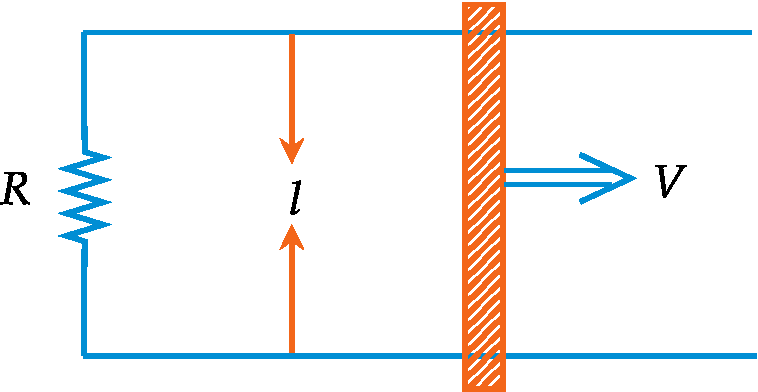
\includegraphics[width=4cm,height=2.5cm]{10-crop}
		\end{center}
	\end{figure}
	\textbf{a)}\quad If the bar moves to the right at  speed $V$ what is the current in the resistor? In what direction does it flow ?\\\\
	\textbf{b)}\quad What is the magnetic force on the bar? In what direction?\\\\
	\textbf{c)}\quad If the bar starts out with a speed $V_0$ at time $f=0$ and is left to slide what is its speed at later time $t$ ?
	\begin{answer}
		Let x be the thickness of the bar,
		\begin{align*}
		\textbf{a)} \quad\phi&=B\cdot A \quad  A=Area=lx\\
		\varepsilon&=\frac{-d \phi}{d t}=-B l \frac{d x}{d t}\\
		&=-B lv \qquad \text{Where,}\ \frac{dx}{dt}=v\\
		\text{But ,}\  \varepsilon&=I R\\
		I R&=B l v\\
		I&=\frac{B l v}{R}
		\end{align*}
		Direction of the current in the bar is given be  Fleming's right hand rule thumb which shows the\\ direction of motion point towards right and forefinger (magnetic field) pointing in to the page.Then current is given by middle finger which points up. So the current flows upward through the bar and downward through the resistor $R$\\
		\begin{align*}
		\textbf{b)}\quad f&=\int(I \times B) \cdot d 1 \quad \theta=90^{\circ}\\
		\text{Here } f&=I B l\hspace{2cm}\text{But,}\  I=\frac{B l v}{R}\\
		&=\frac{B^{2} l^{2} v}{R}\\
		I \times B &\text{ points towards left. } \text{So $F$ to the left.}\\\\
		\textbf{c)}\quad F&=m a= m \frac{ d v}{d t}\\
		m \frac{ d v}{d t}&=\frac{-B^{2} l^{2} v}{R}\\
		\frac{d v}{d t}&=\left(\frac{-B^{2} l^{2}}{R m}\right) v
		\intertext{By solving we get,}
		\therefore v&=v_{0} e^{-{\frac{R^{2} l^{2}}{R m} t}} 
		\end{align*}
	\end{answer}
	\item A square loop of wire (side $a$) lies on a table, a distance $s$ from a very long straight wire, which carries a current $I$\\
	\begin{figure}[H]
		\begin{center}
			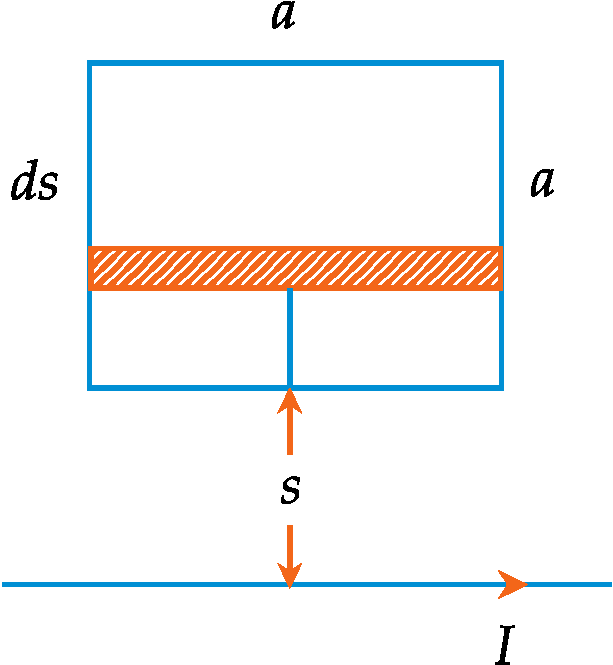
\includegraphics[width=3.5cm,height=3.5cm]{11 01-crop}
		\end{center}
	\end{figure}
	\textbf{a)}\quad Find the flux through the loop?\\\\
	\textbf{b)}\quad Someone pulls the loop directly away foom the wire, at speed $V$, what emf is generated? In what direction does the current flow?\\\\
	\textbf{c)}\quad what if the loop is pulled to the right at speed $V$, instead away?
	\begin{answer}
		\begin{align*}
		\textbf{a)}\hspace{1.9cm} \text{The field }&\text{due to long wire}\\
		B&=\frac{\mu_{0} I}{2 \pi s}\\
		\phi&=\int B \cdot d a\\
		&=\frac{\mu_{0} I}{2 \pi} \int_{s}^{s+a} \frac{1}{s} \times a\  d s\\
		\phi&=\frac{\mu_{0}I a}{2 \pi} \ln \left(\frac{s+a}{s}\right)
		\\\\
		\textbf{b)}\hspace{3cm} \varepsilon&=\frac{-d \phi}{d t}\\
		&=\frac{\mu_{0}I a}{2 \pi} \frac{d}{dt}\ln \left(\frac{s+a}{s}\right)\\
		&=\frac{-\mu_{0} Ia}{2 \pi} \frac{s}{s+a} \left[\frac{\frac{s d s}{d t}-(s+a) \frac{d s}{d t}}{s^{2}}\right]\hspace{2cm}\frac{ds}{dt}=V\\
		&=\frac{-\mu_{0} I a}{2 \pi}\left(\frac{1}{s+a} v-\frac{1}{s} v\right)\\
		\varepsilon&=\frac{\mu_{0} I a^{2} v}{2 \pi s(s+a)}
		\\
		\end{align*}
		The magnetic field due to the wire points out of the page. Therefore the force on the changes at the near side and far side points towards right $(\vec{V}\times\vec{B})$. But field is lener at the far side. So the current flows counterclockwise thoongh the loop.
		\begin{align*}
		\textbf{c)}\quad \text{In this direction there will be no }&\text{flux change. So $\varepsilon=0$}
		\end{align*}
	\end{answer}
	\item A long solenoid with radius $a$ and $n$ turns per unit length carries a time-dependent current $I(t)$ in the $\hat{\phi}$ direction. Find the electric field (magnitude and direction) at a distance $s$ from the axis (both inside and outside ).
	\begin{answer}
		\begin{align*}
		B&=\mu_{0}nI(t) \hspace{1cm} \text{inside}\\
		B&=0\hspace{2cm}\text{outside}\\
		\frac{dB}{dt}&=\mu_{0}n \frac{dI}{dt}\\
		\nabla\times E&=\frac{-dB}{dt}  \frac{dB}{dt}=\mu_{0}n \frac{dI}{dt}\\
		\oint E\cdot dl&=-\int\frac{d}{dt}(B\cdot da)&\oint da=\pi s^2
		\end{align*}
		\textbf{Inside:}\\\\
		Consider an amperian loop of radius of $s$ \quad $s<a$
		\begin{align*}
		E\times2\pi s=\mu_{0}n \frac{dI}{dt}\times\pi s^2\\
		E=\frac{\mu_{0}n s}{2}\frac{dI}{dt}\hat{\phi}
		\end{align*}
		\textbf{Outside:}\\
		\opencutright
		\renewcommand\windowpagestuff{
			\centering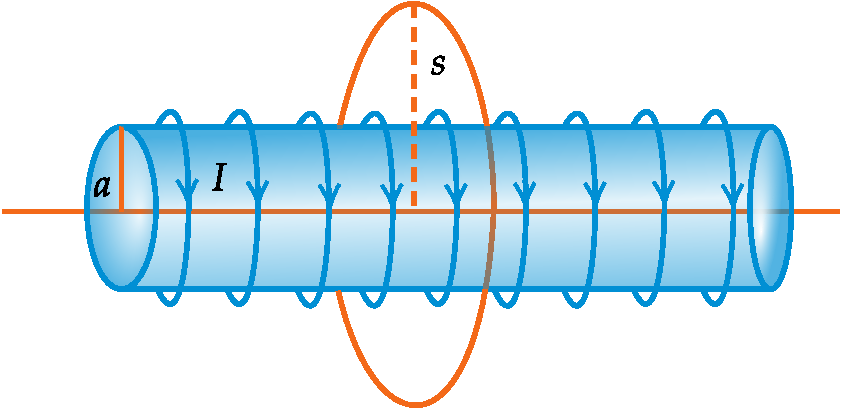
\includegraphics[width=6cm]{diagram-20210426(7)-crop}}
		\begin{cutout}{3}{\dimexpr\linewidth-12cm\relax}{0pt}{4}
			\begin{align*}
			\oint E\cdot dl&=-\int\frac{d}{dl}B.da\\
			&=\frac{-d \phi}{dt}\\
			\oint B\cdot da&=\mu_{0}I(t)\times\pi a^2\\
			E\times2\pi s&=\mu_{0} n\times\pi a^2 \frac{dI}{dt}\\
			E&=\frac{-\mu_{0}n a^2}{2 s} \frac{dI}{dt}\hat{\phi}
			\end{align*}
		\end{cutout}
	\end{answer}
	\item Find the self-inductance of a toroidal coil with rectangular cross section (inner radius $a$, outer radius $b$, height $h$ ), which carries a total of $N$ turns.
	\begin{answer}
		The magnetic field inside the toroid is\\ 
		\opencutright
		\renewcommand\windowpagestuff{
			\centering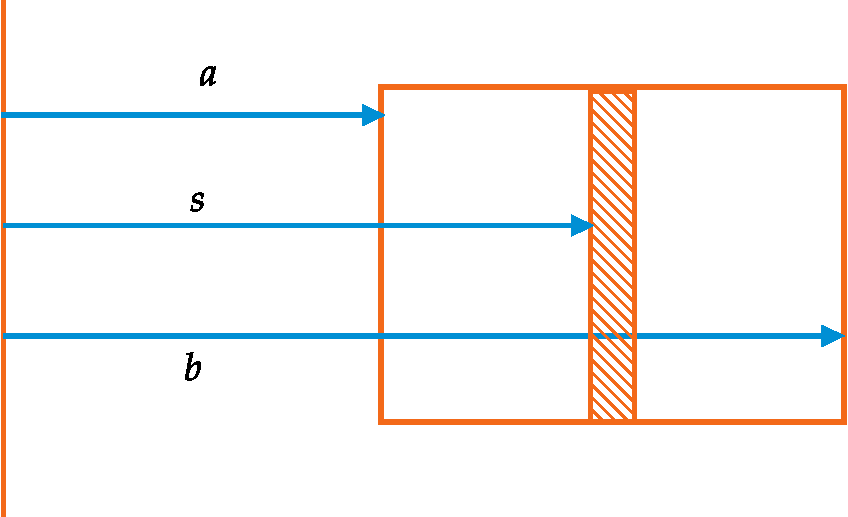
\includegraphics[width=4cm]{diagram-20210426(4)-crop}}
		\begin{cutout}{3}{\dimexpr\linewidth-7cm\relax}{0pt}{4}
			\begin{align*}
			B&=\frac{\mu_{0}N I}{2\pi s}\\
			\text{The flux through a single turn}\\
			\phi&=\int {B} \cdot d \mathbf{a}\\
			&=\frac{\mu_{0} N I}{2 \pi} h \int_{a}^{b} \frac{1}{s} d s\\
			&=\frac{\mu_{0} N I h}{2 \pi} \ln \left(\frac{b}{a}\right)\\
			\text{Total flux through $N$ single turns}\\
			\phi&=\frac{\mu_{0} N^{2} h}{2 \pi} \ln \left(\frac{b}{a}\right)\times I\\
			L&=\frac{\mu_{0} N^{2}  N}{2 \pi} \ln \left(\frac{b}{a}\right)
			\end{align*}
		\end{cutout}
		
	\end{answer}
	\item A small loop of wire (radius $a$ ) lies a distance $z$ above the center of a large loop (radius $b$ ). The planes of the two loops are parallel, and perpendicular to the common axis. \\
	\begin{minipage}{.45\textwidth}
		\begin{center}
			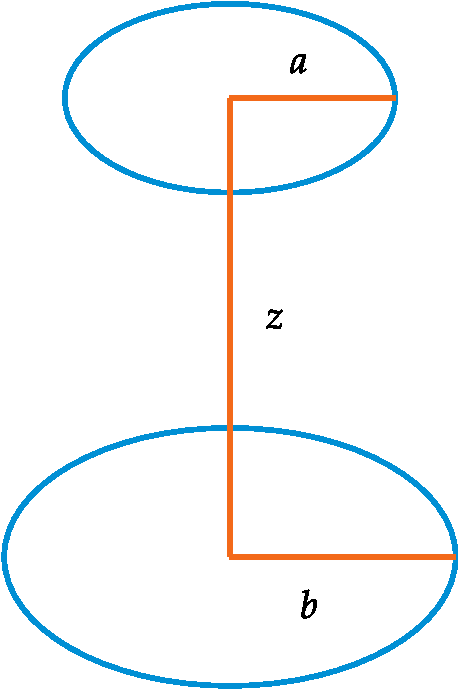
\includegraphics[width=0.3\textwidth]{diagram-20210426(5)-crop}
		\end{center}
	\end{minipage}\\\vspace{.2cm}\\
	\textbf{(a)} Suppose current $I$ flows in the big loop. Find the flux through the little loop. (The little loop is so small that you may consider the field of the big loop to be essentially constant.)\\
	\textbf{(b)} Suppose current $I$ flows in the little loop. Find the flux through the big loop. \\
	\textbf{(c)} Find the mutual inductance, and confirm that, $M_{12}=M_{21}$.
	\begin{answer}
		\textbf{(a)}
		\begin{align*}
		\phi&=\int B.da\\
		B&=\frac{\mu_{0}I}{2}\frac{b^2}{(b^2+z^2)^\frac{3}{2}}\hspace{1cm}\text{At little loop due to big loop}\\
		da&=\pi a^2\\
		\phi&=\frac{\mu_{0}I}{2}\frac{b^2}{(b^2+z^2)^\frac{3}{2}}\times\pi a^2\\
		&=\frac{\mu_{0}\pi a^2 b^2}{2(b^2+z^2)^\frac{3}{2}}
		\end{align*}
		\textbf{(b)} \quad Here the little loop can be consider as a magnetic dipole of magnetic moment \\
		$$ M=IA=I\pi a^2$$\\
		Field at bigloop due this $M$ is\\ 
		$$ B=\frac{\mu_{0}}{4\pi}\frac{M}{r^3}(2\cos\theta\hat{r}+\sin\theta\hat{\theta})$$\\
		\begin{flushright}
			\begin{minipage}{.45\textwidth}
				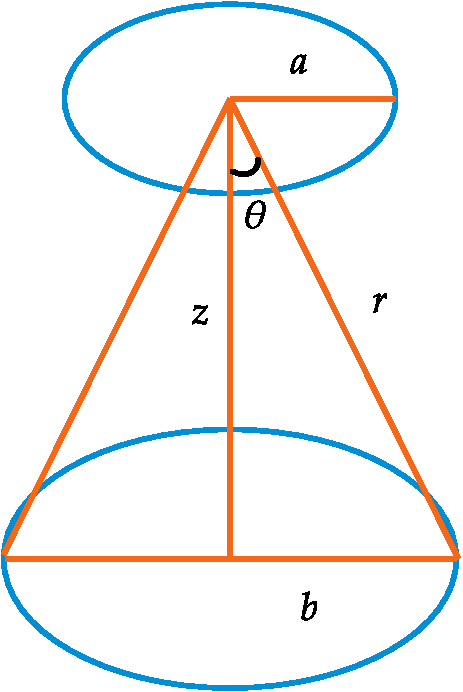
\includegraphics[width=0.4\textwidth]{diagram-20210426(6)-crop}
			\end{minipage}\\
		\end{flushright}
		There is no component in the direction of magnetic dipole.\\  
		\begin{minipage}{0.60\textwidth}\hfill
			\begin{align*}
			\text{so, }  \phi&=\int B\cdot da\\
			\phi&=\frac{\mu_{0}}{4 \pi}\frac{M}{r^3}\int2\cos\theta r^2\sin\theta d\theta d\phi\\
			\phi&=\frac{\mu_{0}}{4\pi}\frac{2M}{r}\times2\pi\int_0\cos\theta\sin\phi d\theta\\
			&=\frac{\mu_{0}M}{r}\frac{\sin^2\theta}{2}\\
			&=\frac{\mu_{0}I\pi a^2 b^2}{2(b^2+z^2)^\frac{3}{2}}\\
			&\text{so $\phi$ is same in both cases}
			\end{align*}
		\end{minipage}
		\begin{minipage}{0.40\textwidth}
			\begin{align*}
			da=r^2\sin\theta d\theta d\phi\hat{r}\\
			\int^{2\pi}_0 d\phi=2\pi\\
			\cos\theta=z\\
			\sin\theta=\frac{b}{r}\\
			r=\sqrt{b^2+z^2}\\
			M=I\pi a^2
			\end{align*}
		\end{minipage}
		\textbf{(c)}
		\begin{align*}
		\phi&=MI\\
		\therefore M&=\frac{\mu\pi a^2 b^2}{2(b^2+z^2)^\frac{3}{2}}\\ &\text{since\ $\phi$'s are same}\\
		M_{21}&=M_{12}
		\end{align*}
	\end{answer}
	
\end{enumerate}



